%% main.tex adaptado para o template Inf da UFRGS
%% Conteúdo original de João Vitor Spolavore e Thiago Gonçalves
%
% This work may be distributed and/or modified under the
% conditions of the LaTeX Project Public License, either version 1.3
% of this license or (at your option) any later version.
% The latest version of this license is in
%   http://www.latex-project.org/lppl.txt
% and version 1.3 or later is part of all distributions of LaTeX
% version 2005/12/01 or later.

\documentclass{beamer}

\usepackage[T1]{fontenc}
\usepackage[brazil]{babel}
\usepackage[utf8]{inputenc}
\usepackage{hyperref}
\usepackage{booktabs} % For better tables
\usepackage{graphicx}
\usepackage{booktabs} 
\usepackage{multirow}

% Choose the Inf theme
\usetheme{Inf}

% Define the title with \title[short title]{long title}
\title[Comparação PageRank]{Comparação entre PageRank Sequencial e Paralelizado}

\date{\today}

% Author information
\author{João Vitor Spolavore \and Thiago Gonçalves}
\institute{Instituto de Informática --- UFRGS}

\begin{document}

% Command to create title page
\InfTitlePage

\begin{frame}
  \frametitle{Agenda}
  \tableofcontents
\end{frame}

\section{Introdução}
\begin{frame}{Introdução}
    O presente relatório tem por objetivo apresentar o efetivo progresso realizado pelos estudantes João Vitor Spolavore e Thiago Gonçalves da análise comparativa entre o algoritmo PageRank Sequencial e sua versão Paralela.\\
    \vspace{0.5em}
    Ainda, explicaremos como o projeto foi realizado, as decisões tomadas, as escolhas de parâmetros, os resultados até o momento e, por fim, citar as dificuldades enfrentadas ao longo do projeto.
\end{frame}

\section{Ambiente de Teste}
\begin{frame}{Máquina Utilizada}
    Todos os experimentos realizados foram executados no Parque de Computação de Alto Desempenho (PCAD) da Universidade Federal do Rio Grande do Sul (UFRGS).
    Utilizamos o nó computacional denominado \textit{blaise}.

    \subsection*{Características da Máquina}
    \begin{itemize}
        \item \textbf{Nome:} blaise
        \item \textbf{CPU:} 2 x Intel(R) Xeon(R) E5-2699 v4, 2.20 GHz, 88 threads, 44 cores
        \item \textbf{RAM:} 256GB 
        \item \textbf{Disco:} 1.8 TB SSD, 1.8 TB HDD
        \item \textbf{Placa mãe:} Supermicro X10DGQ
    \end{itemize}
    \url{https://gppd-hpc.inf.ufrgs.br}\\
    \vspace{0.6em}
    Esta máquina possui DOIS processadores Intel, fundamental para a escolha devido às possibilidades de experimentos com distribuição de threads.
\end{frame}

\section{Método de análise e coleta de dados}
\begin{frame}{Método de análise}
    Como citado na Etapa 1, o presente projeto apresenta uma perspectiva de medição para o método de análise.\\
    \vspace{0.5em}
    Para ajudar nessa abordagem, utilizamos o Intel Vtune Profiler para coletar os dados da aplicação - gerando um relatório em formato \textit{csv} ao final da execução. Decidimos utilizar essa ferramenta pois:
    \vspace{0.5em}
    \begin{itemize}
        \item O grupo já possuia uma breve experiência com ela.
        \item Os processadores presentes na máquina escolhida eram Intel.
        \item É uma ferramenta amplamente utilizada pela própria Intel para obter métricas de seus processadores.
    \end{itemize}
\end{frame}
\begin{frame}{Análise do Vtune - Pontos positivos}
        \begin{itemize}
        \item Fácil configuração.
            \begin{itemize}
                \item 1 comando para carregar as variáveis.
                \item 1 comando para realizar a coleta.
                \item 1 comando para realizar a sumário em csv.
            \end{itemize}
        \vspace{0.5em}
        \item Integração simples com o objeto de análise.
        \vspace{0.5em}
        \item Diretórios de output configuráveis.
    \end{itemize}
\end{frame}
\begin{frame}{Análise do Vtune - Pontos negativos}
        \begin{itemize}
        \item Arquivos de saída mal formatados.
        \vspace{0.5em}
        \item Overhead considerável e diferente entre os tipos de análise.
        \vspace{0.5em}
        \item Excesso de arquivos gerados no final da análise.
    \end{itemize}

\end{frame}

\begin{frame}{Análise do Vtune}
    Com isso tudo, consideramos que foi uma escolha adequada e facilitou consideravelmente o processo de coleta de dados.
\end{frame}

\begin{frame}{Definição dos experimentos}
    Escolhemos utilizar o governor DVFS \textit{performance} com o comando \texttt{cpufreq-set -g performance}. \\
    \vspace{0.5em}
    A fim de centralizar todos as instâncias dos experimentos desejados e automatizar o processo de execução através de scripts, criamos um csv contendo a definição de todos os nossos experimentos denominado experiments.csv.\\
    \vspace{0.5em}
    Além disso, executamos cada configuração 5 vezes pra garantir a robustez dos nossos resultados e também evitar o impacto de possíveis outliers na nossa pesquisa.
    Por fim, para essa etapa focamos nas métricas de tempo total gasto, speed up e eficiência do paralelismo.
\end{frame}
\begin{frame}{Definição dos experimentos}
    \begin{itemize}
        \item \textbf{Quantidade de instâncias:} 757.
        \item \textbf{Quantidade de execuções:} 757 * 5 = 3785.
         \item \textbf{Quantidade de colunas no arquivo:} 9.
    \end{itemize}
    \vspace{0.5em}
    Conteúdo completo do arquivo de experimentos: \\ \url{https://github.com/thgdsg/perf-analysis/blob/main/stage2/experiments.csv}
\end{frame}

\begin{frame}{Parâmetros Considerados}
    Consideramos as seguintes opções para análise:
    \begin{itemize}
        \item \textbf{Número de Threads}: {1, 4, 12, 22, 28, 36, 44, 66, 88}.
        Abrange threads físicas (22), lógicas/totais por CPU (44), e total da máquina (88).
        \item \textbf{Tipo de Análise feita pelo Profiler}: {hpc-performance, hotspots, performance-snapshot}.
        Importante para obter informações sobre gasto de tempo, eficácia da paralelização e uso/atribuição de threads.
    \end{itemize}
\end{frame}



\begin{frame}{Parâmetros Considerados (cont.)}
    \begin{itemize}
        \item \textbf{Estado do Hyperthreading (ON/OFF)}: Com o objetivo de avaliar o impacto no desempenho, forçamos 1 thread por core com a variável \texttt{OMP\_PLACES=cores/threads} e reduzimos visibilidade de threads lógicas com \texttt{GOMP\_CPU\_AFFINITY} e o comando \texttt{taskset -c [NÚMEROS DOS CORES]}.
        \item \textbf{Política de \textit{Binding} de Threads}: Analisa o impacto da distribuição de threads entre os dois processadores via \texttt{OMP\_PROC\_BIND} com essas opções:
        \begin{itemize}
            \item \texttt{close}: Vincula threads a lugares próximos à thread pai, útil para localidade de cache.
            \item \texttt{spread}: Distribui threads em partições mais distantes, útil para reduzir contenção em recursos compartilhados.
        \end{itemize}
    \end{itemize}
\end{frame}

\begin{frame}{Análises do V-tune}
    \begin{itemize}
    \item \textbf{hpc-performance}: Essa análise coleta métricas detalhadas de uso de hardware, como largura de banda de memória, eficiência de cache, paralelismo de instruções (ILP) e balanceamento entre threads, ajudando a identificar gargalos em aplicações fortemente paralelas.
    
    \item \textbf{hotspots}: Essa análise é útil para detectar funções ou loops críticos e orientar otimizações de desempenho no nível do código-fonte.
    
    \item \textbf{performance-snapshot}: Fornece uma visão geral automática do desempenho da aplicação. Ele realiza uma coleta rápida de métricas-chave — como utilização da CPU, eficiência de paralelismo, uso de memória e E/S.
    \end{itemize}
\end{frame}

\begin{frame}{Scripts e Automações}
    Scripts utilizados para automatizar execução e análise:
    \begin{itemize}
        \item \texttt{perf\_analysis\_pr.sh}: Orquestração local (prepara ambiente, carrega VTune, executa comandos).
        \item \texttt{run.slurm}: Execução em cluster SLURM.
        \item \texttt{src/build\_commad.py}: Geração da matriz de execuções de \texttt{experiments.csv} para \texttt{src/commands.sh}.
        \item \texttt{src/commands.sh}: Script gerado com todas as combinações de execuções.
        \item \texttt{src/unify\_all\_results.py}: Pós-processamento (extrai tempo, calcula speedup e eficiência, unifica em \texttt{unified\_results.csv}).
        \item \texttt{src/execute\bench.sh}: Executa uma instância específica. Recebe os parâmetros presentes no experiments.csv, configura as variáveis de ambiente do OpenMP, criar os diretórios de output e chama o comando do vtune para coleta e sumário de dados.
    \end{itemize}
\end{frame}

\begin{frame}{Scripts e Automações (cont.)}
    \textbf{Fluxo Resumido}
    \begin{enumerate}
        \item Preparação do ambiente
        \item Geração de comandos a partir de \texttt{experiments.csv}
        \item Execução sistemática
        \item Coleta em \texttt{results/}
        \item Unificação em \texttt{unified\_results.csv}
    \end{enumerate}

    \textbf{Entrada:} \texttt{experiments.csv}.\\
    \textbf{Saídas:} Diretório \texttt{results/} e \texttt{unified\_results.csv} juntando todos resultados em um csv.
    
    Visamos obter o máximo de reprodutibilidade, minimizar o impacto de \textit{outliers}, e ter uma limpeza de resultados.
\end{frame}

\section{Algoritmo e Dados}

\begin{frame}
    \frametitle{Algoritmo e Fonte de Dados}

    \begin{itemize}
        \item \textbf{Algoritmo:} Utilizamos uma implementação consolidada do PageRank do repositório GAPBS (\url{https://github.com/sbeamer/gapbs}).
        \item \textbf{Fonte dos Dados:} Os grafos foram obtidos da \textit{Stanford Large Network Dataset Collection} (SNAP), um repositório consagrado academicamente (\url{https://snap.stanford.edu/data/index.html}).
        \item \textbf{Requisito:} Para executar o algoritmo PageRank, a aplicação recebe como entrada grafos \textbf{direcionados}.
    \end{itemize}
\end{frame}

\begin{frame}
    \frametitle{Grafos Utilizados}

    A tabela abaixo detalha as redes de grafos escolhidas para os experimentos:

    \centering
    \begin{tabular}{lrr}
        \toprule
        \textbf{Grafo} & \textbf{Vértices} & \textbf{Arestas} \\
        \midrule
        Friendster     & 65,608,366        & 1,806,067,135    \\
        LiveJournal    & 3,997,962         & 34,681,189       \\
        Orkut          & 3,072,441         & 117,185,083      \\
        BerkStan       & 685,230           & 7,600,595        \\
        Google         & 875,713           & 5,105,039        \\
        NotreDame      & 325,729           & 1,497,134        \\
        Stanford       & 281,903           & 2,312,497        \\
        \bottomrule
    \end{tabular}

    \vspace{1em} % Adiciona um espaço vertical
    Todos representam conexões entre páginas web e/ou redes sociais e são dados do mundo real.

\end{frame}

\section{Resultados}

\begin{frame}
    \frametitle{Explicação dos Gráficos de Speedup}
        Agora, mostraremos os gráficos de \textit{speedup}.
        O speedup é quão mais rápido a versão paralela foi comparado a versão sequencial. 
        
        Os gráficos a seguir estão organizados da esquerda pra direita:
        \begin{itemize}
            \item Tipo de Análise performance-snapshot
            \item Tipo de Análise hotspots
            \item Tipo de Análise hpc-performance
        \end{itemize}

        E com 4 possíveis organizações:
        \begin{enumerate}
            \item Hyperthreading Desligado, Política Spread - HT\_OFF\_spread
            \item Hyperthreading Ligado, Política Spread - HT\_ON\_spread
            \item Hyperthreading Desligado, Política Close - HT\_OFF\_close
            \item Hyperthreading Ligado, Política Close - HT\_ON\_close
        \end{enumerate}
\end{frame}

\begin{frame}
    \frametitle{Speedup - Friendster}

    \begin{figure}
        \centering
        \makebox[\textwidth][c]{%

            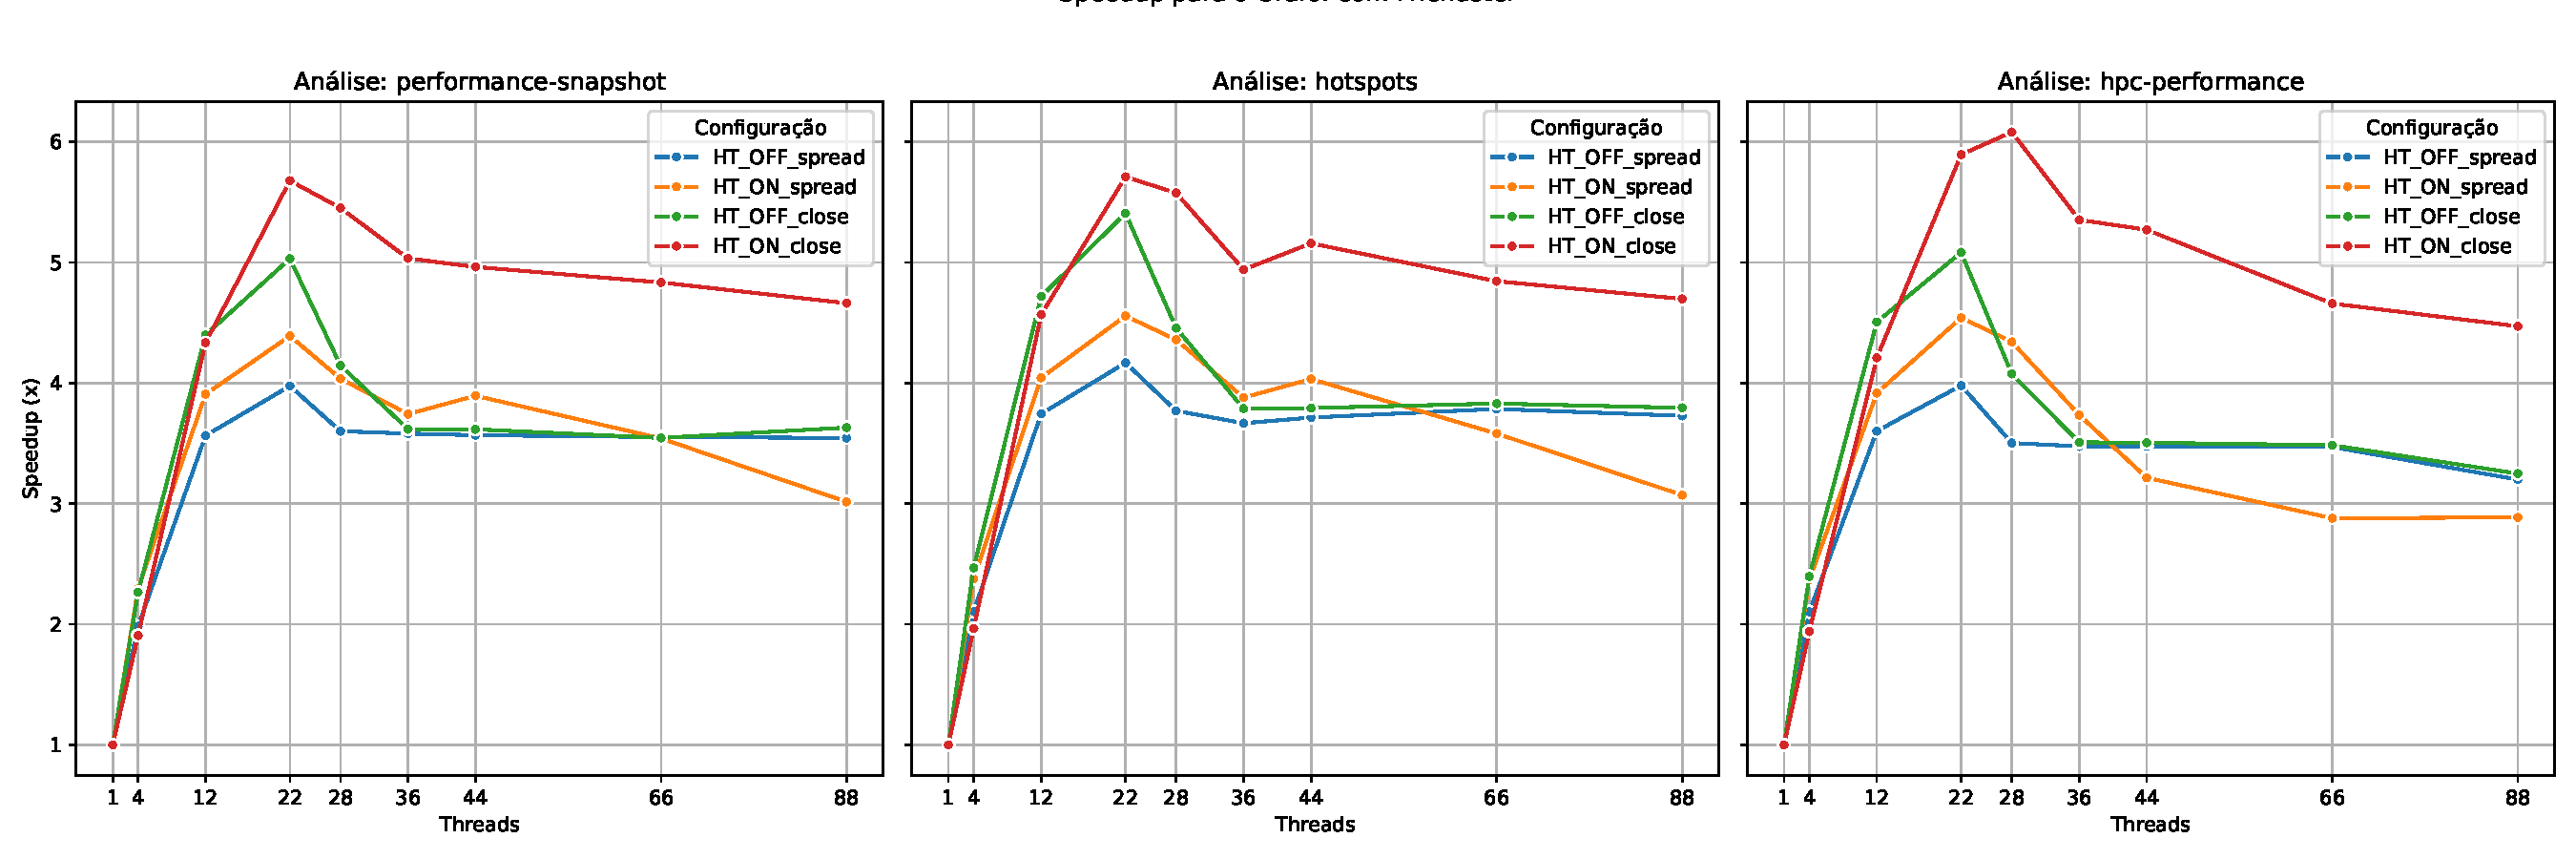
\includegraphics[width=0.95\paperwidth]{graficos/speedup_com-Friendster.pdf}
        }
    \end{figure}
    % insira comentario aqui
    \centering
    No maior grafo, o Hyperthreading Ligado com a política "close" (HT\_ON\_close) obteve melhor speedup em quase todos os casos.
\end{frame}

\begin{frame}
    \frametitle{Speedup - LiveJournal}

    \begin{figure}
        \centering
        \makebox[\textwidth][c]{%
            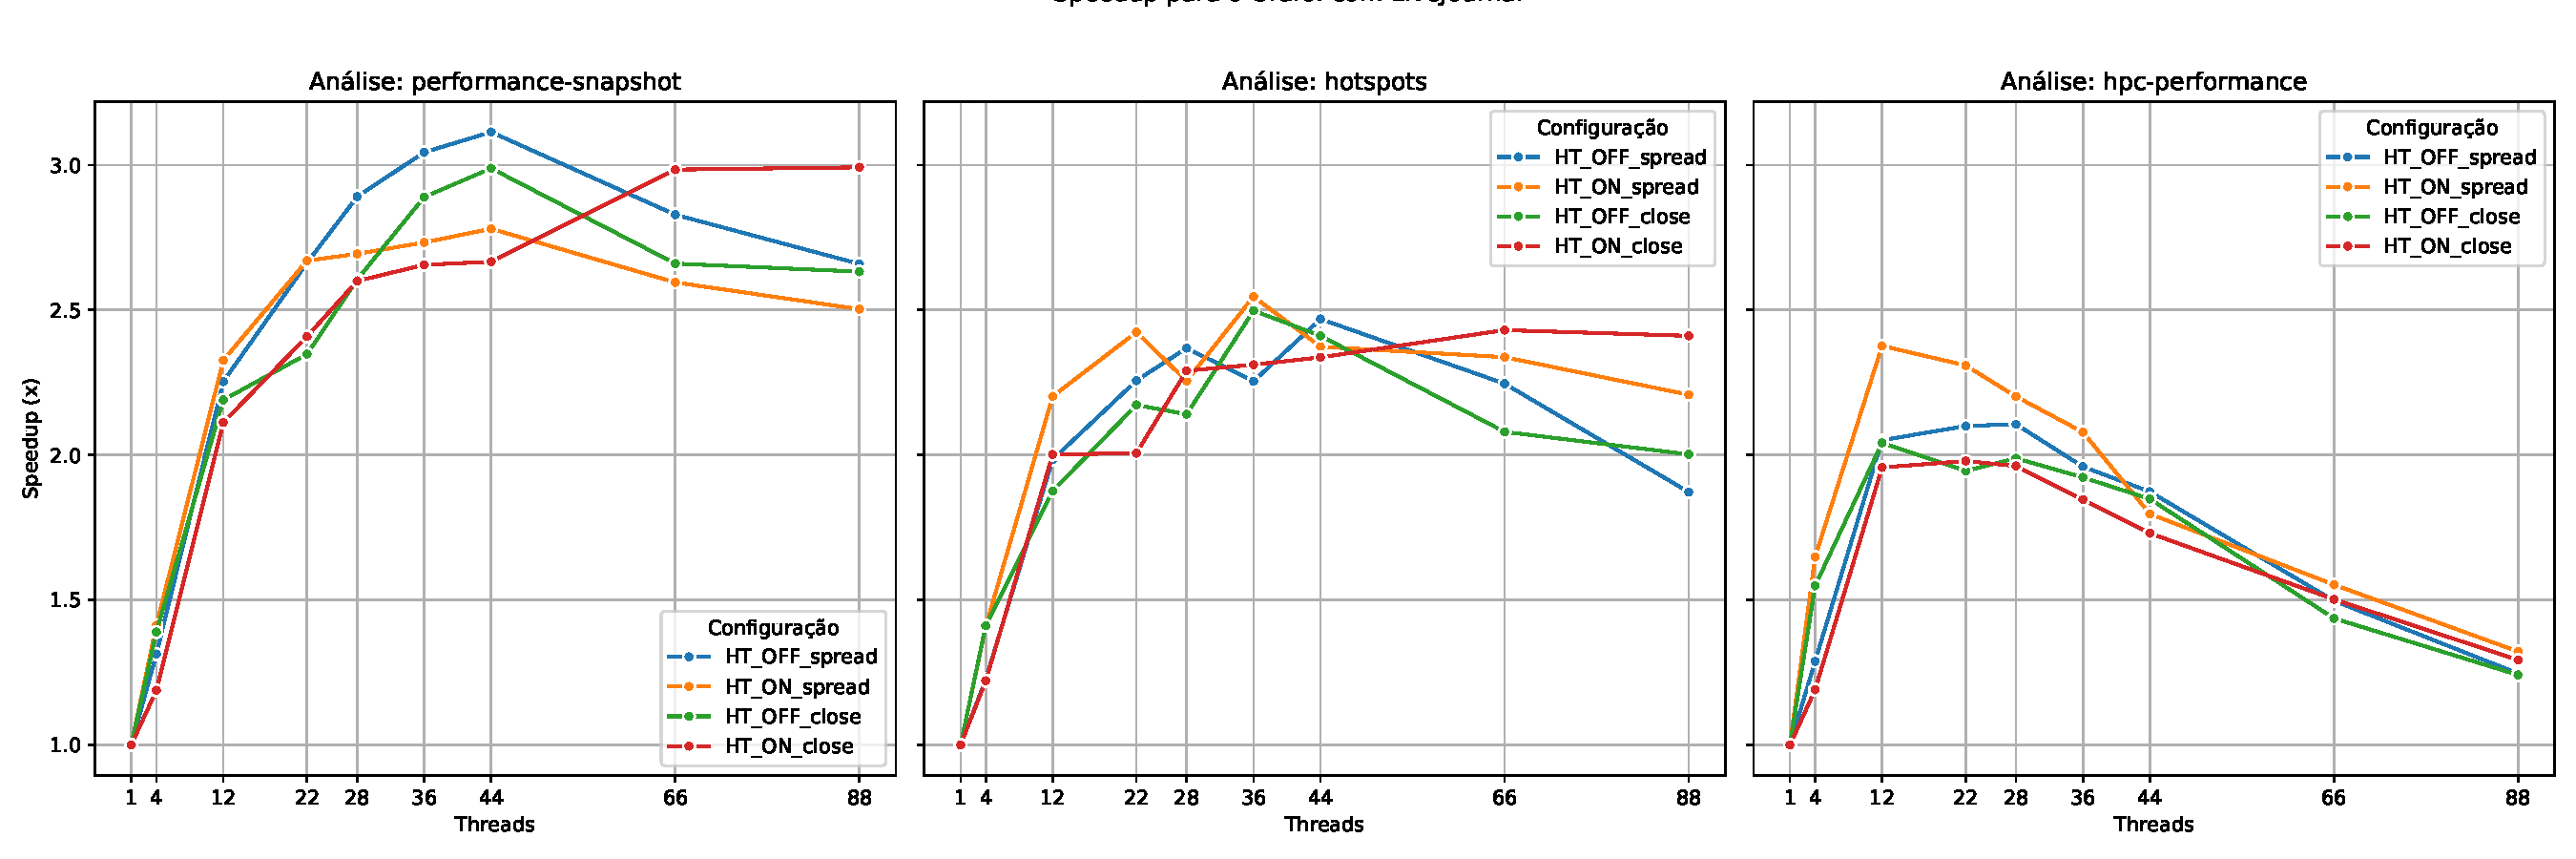
\includegraphics[width=0.95\paperwidth]{graficos/speedup_com-LiveJournal.pdf}
        }        
    \end{figure}
    \centering
    Nesse grafo de tamanho mais modesto, as outras configurações além da HT\_ON\_close conseguiram obter speedup maior com menos threads.
\end{frame}

\begin{frame}
    \frametitle{Speedup - Orkut}

    \begin{figure}
        \centering
        \makebox[\textwidth][c]{%

            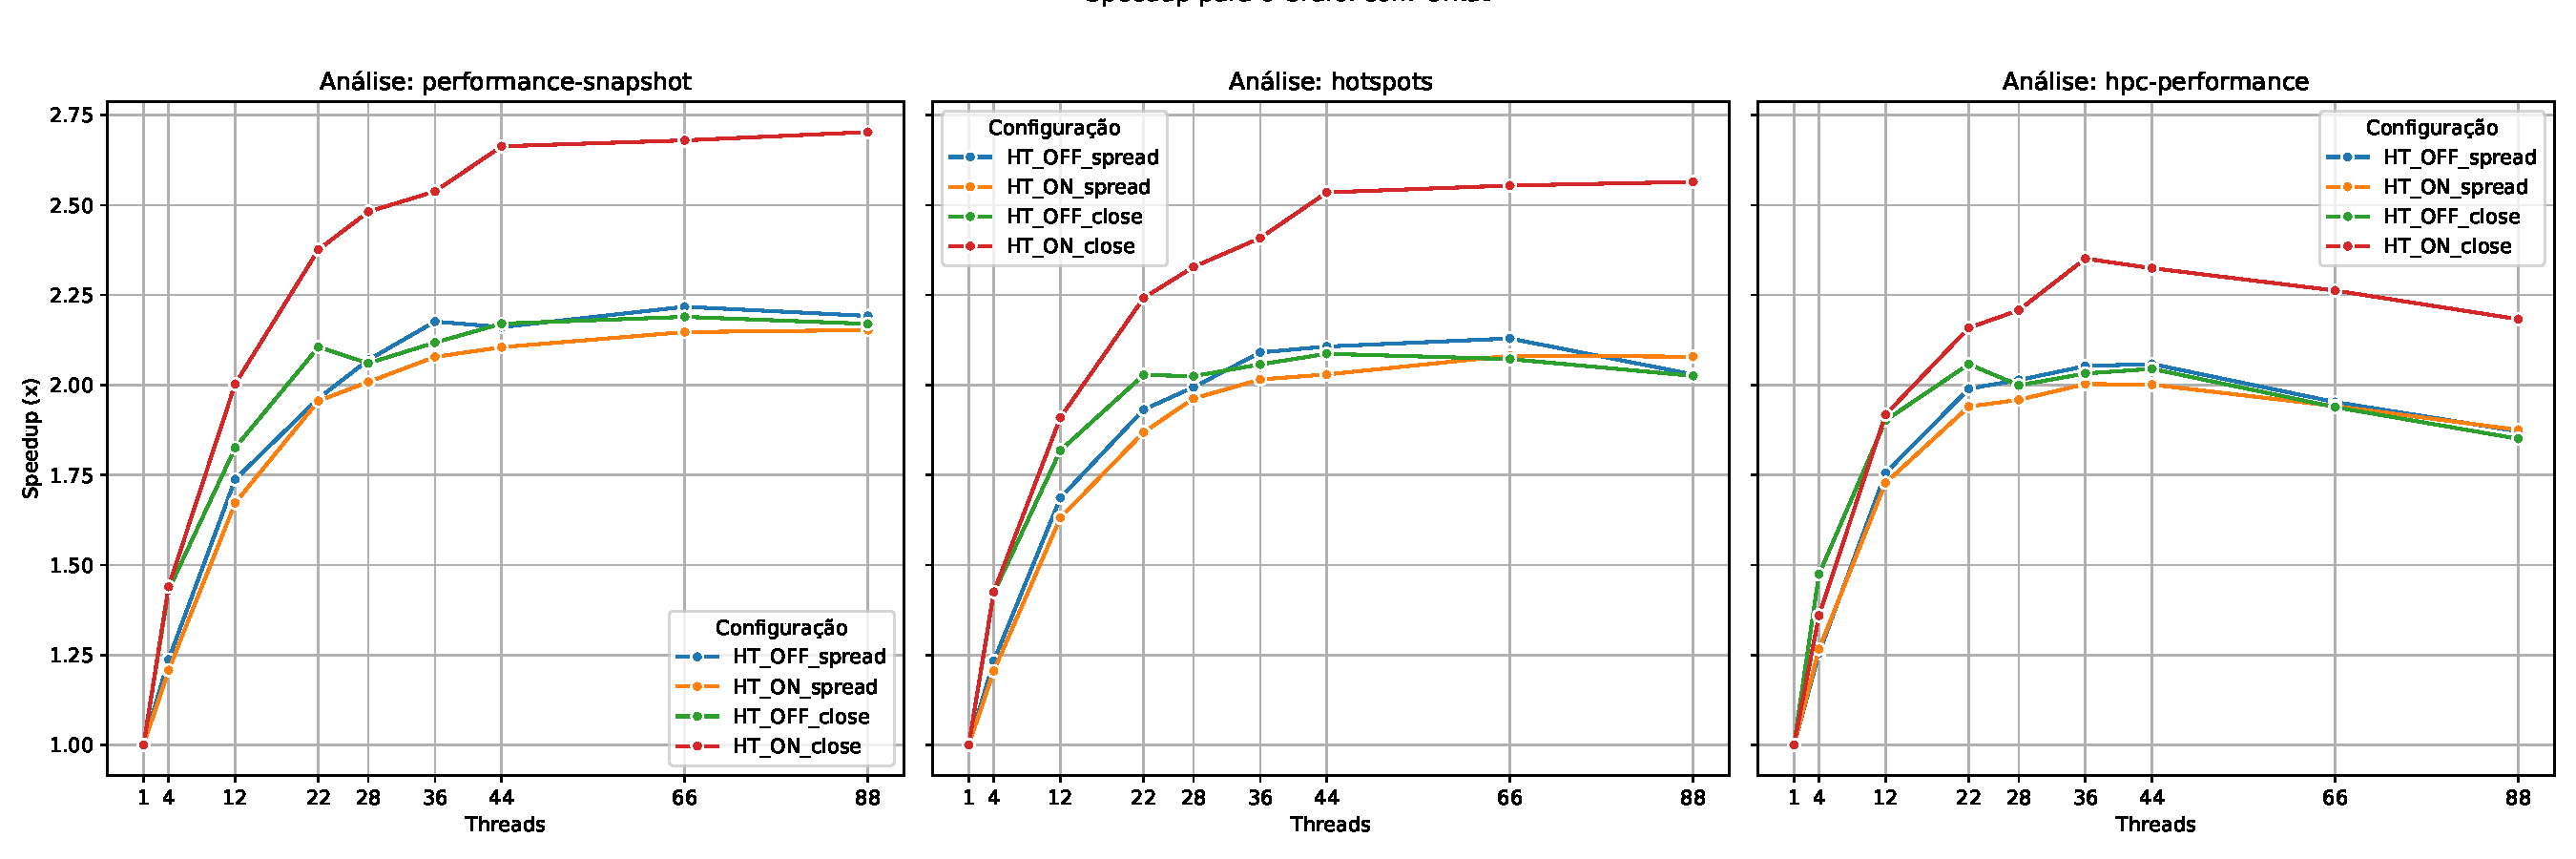
\includegraphics[width=0.95\paperwidth]{graficos/speedup_com-Orkut.pdf}
        }        
    \end{figure}
    \centering
    A configuração HT\_ON\_close foi melhor em todos os casos.
\end{frame}

\begin{frame}
    \frametitle{Speedup - BerkStan}

    \begin{figure}
        \centering
        \makebox[\textwidth][c]{%

            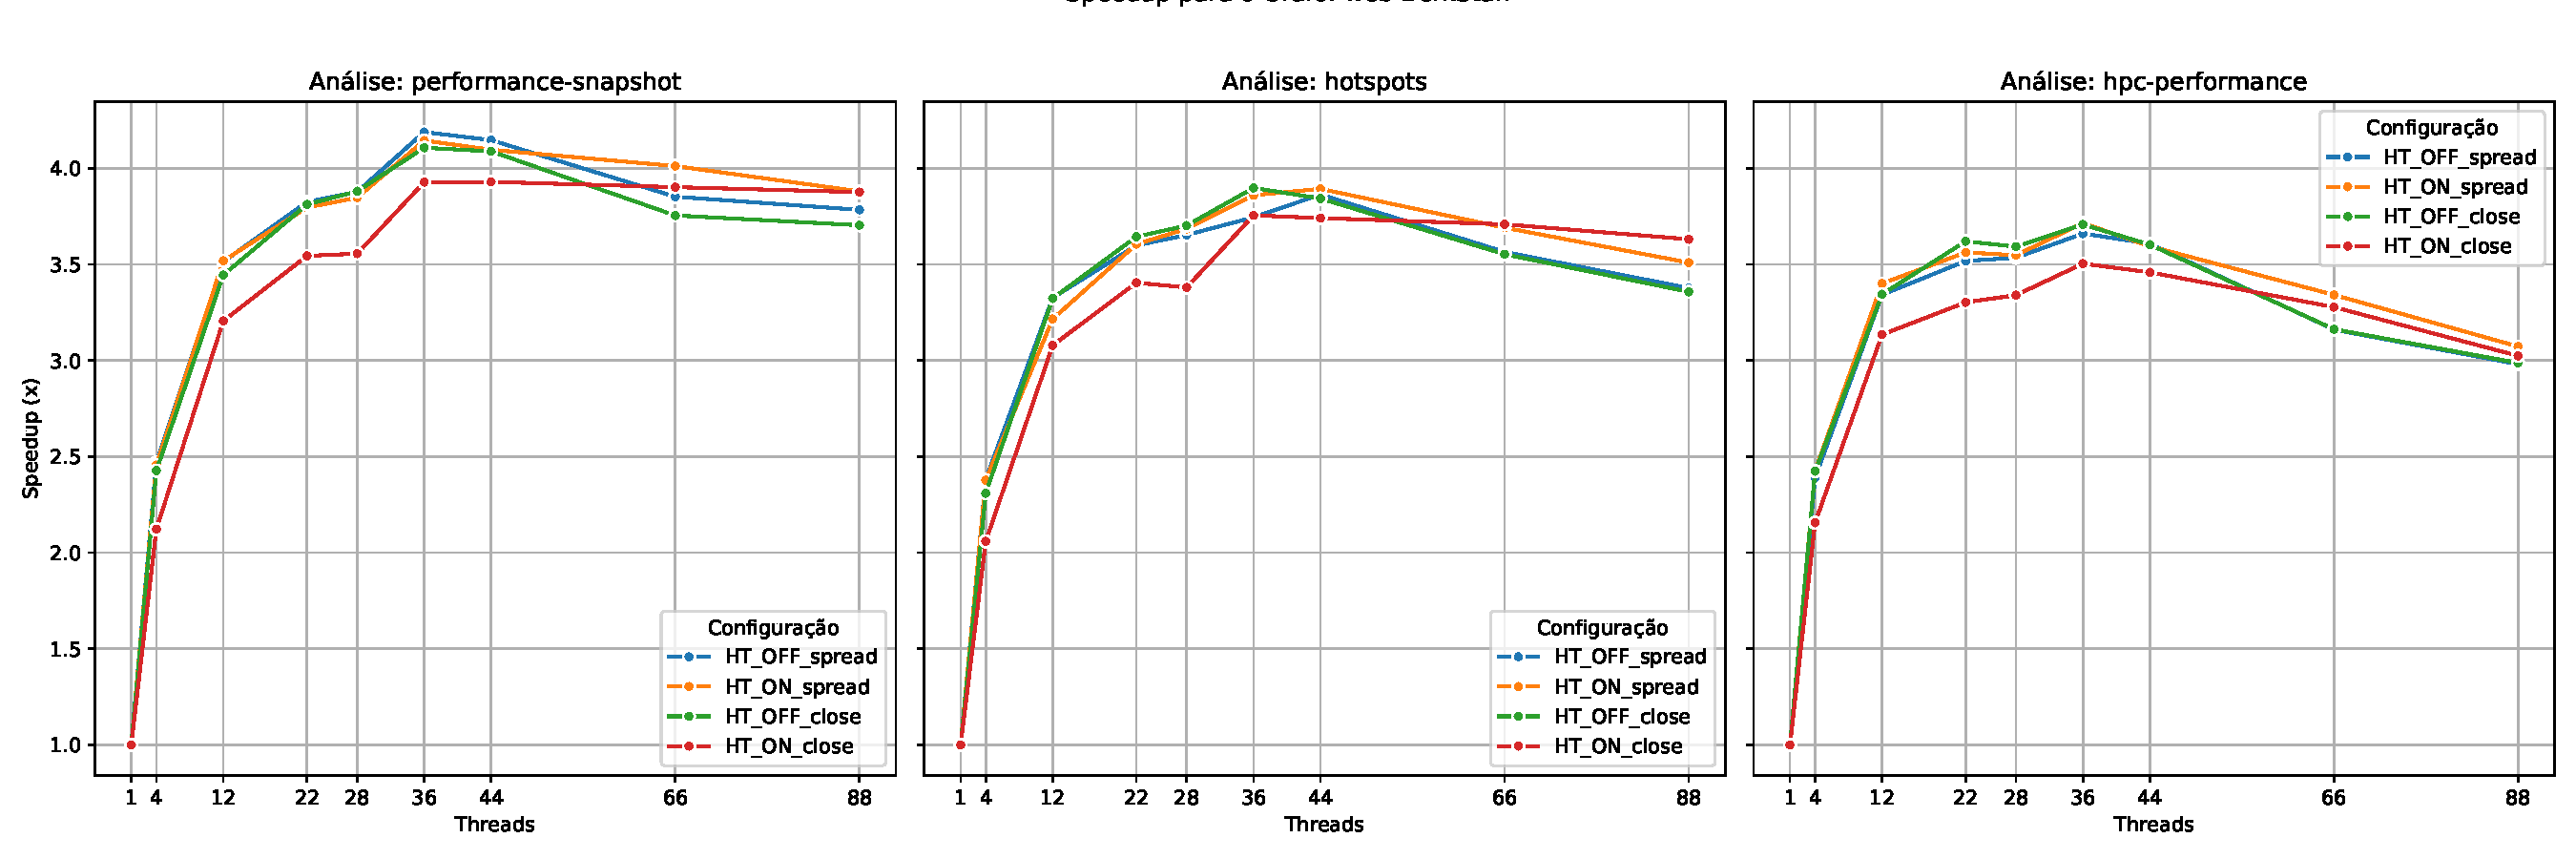
\includegraphics[width=0.95\paperwidth]{graficos/speedup_web-BerkStan.pdf}
        }        
    \end{figure}
    \centering
    Resultados mistos, não houve nenhuma que se destacou, mas o speedup da HT\_ON\_close foi menor com menos threads.
\end{frame}

\begin{frame}
    \frametitle{Speedup - Google}

    \begin{figure}
        \centering
        \makebox[\textwidth][c]{%

            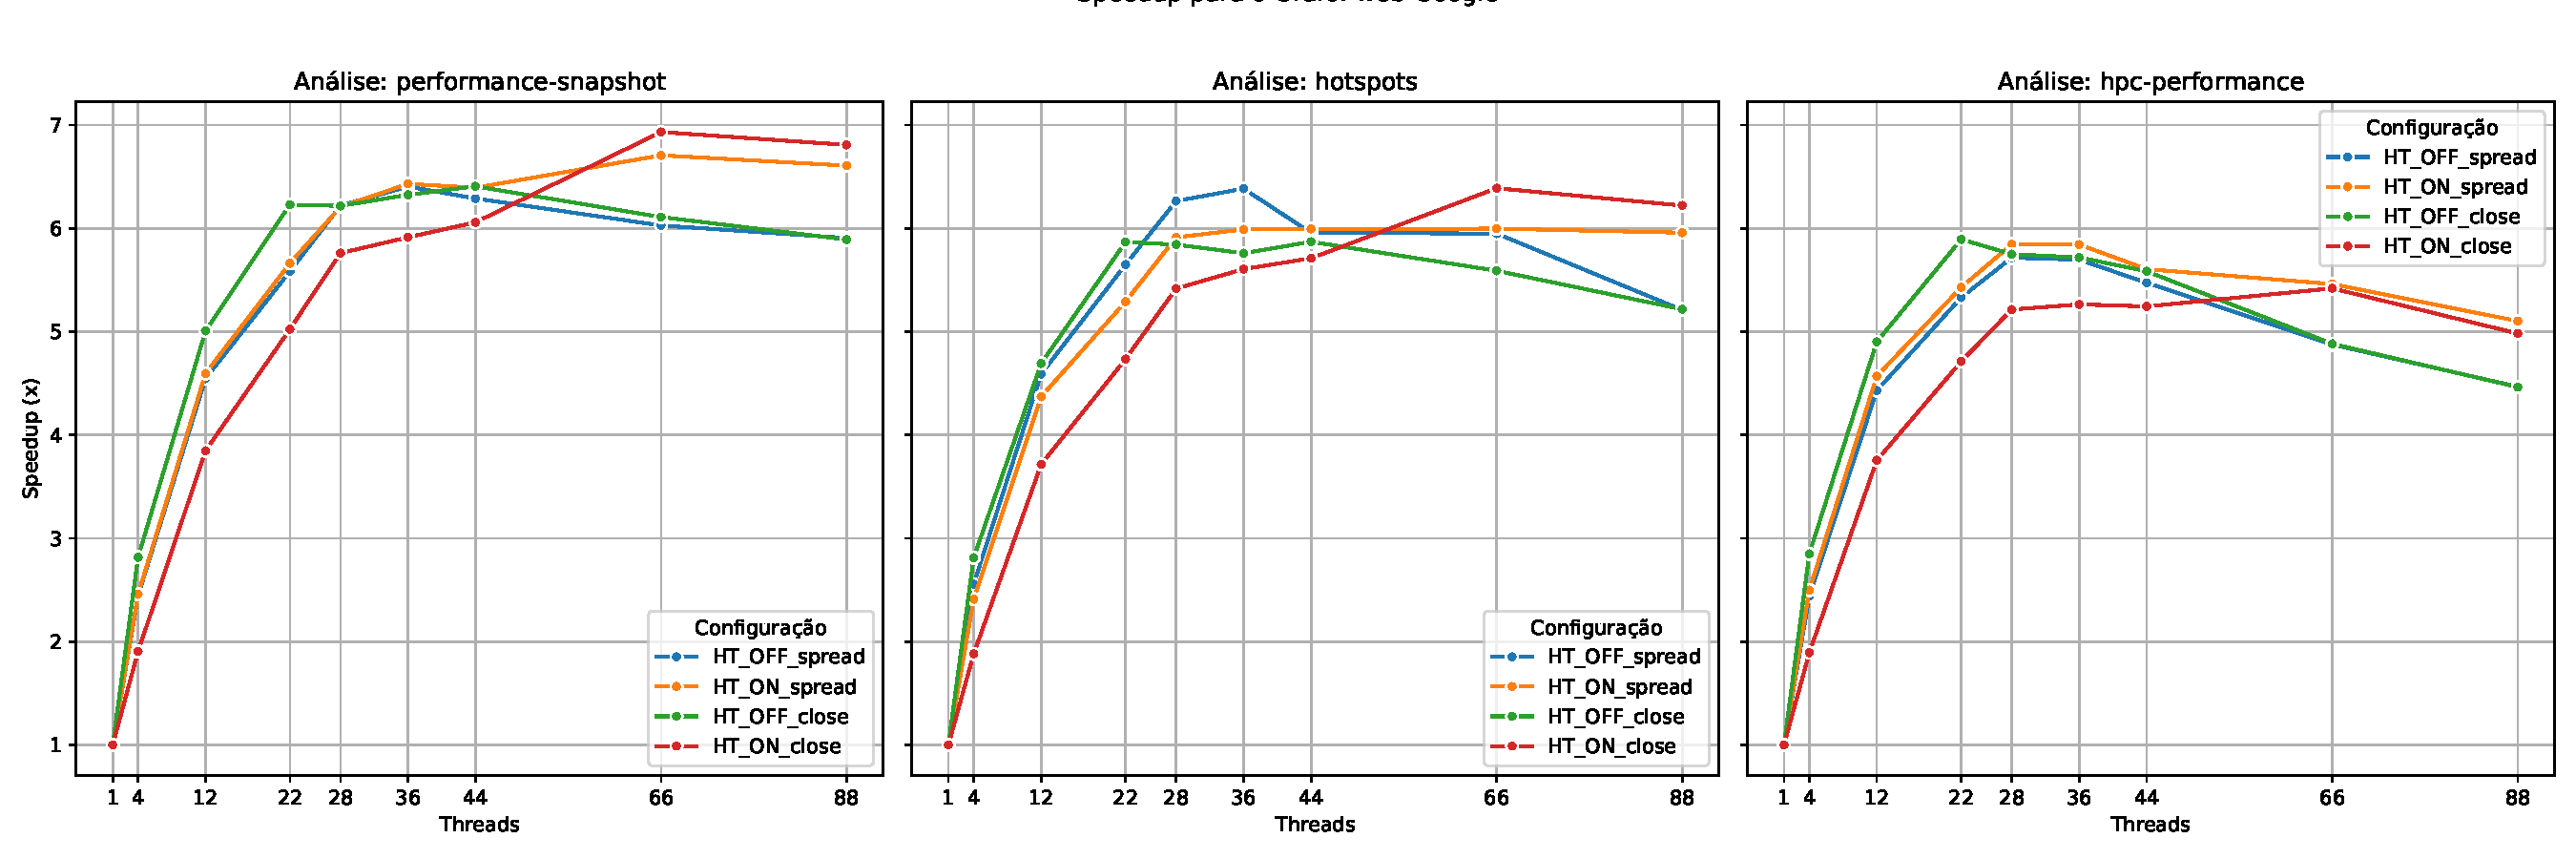
\includegraphics[width=0.95\paperwidth]{graficos/speedup_web-Google.pdf}
        }        
    \end{figure}
    \centering
    Novamente, a HT\_ON\_close se saiu melhor com mais threads.
\end{frame}

\begin{frame}
    \frametitle{Speedup - NotreDame}

    \begin{figure}
        \centering
        \makebox[\textwidth][c]{%

            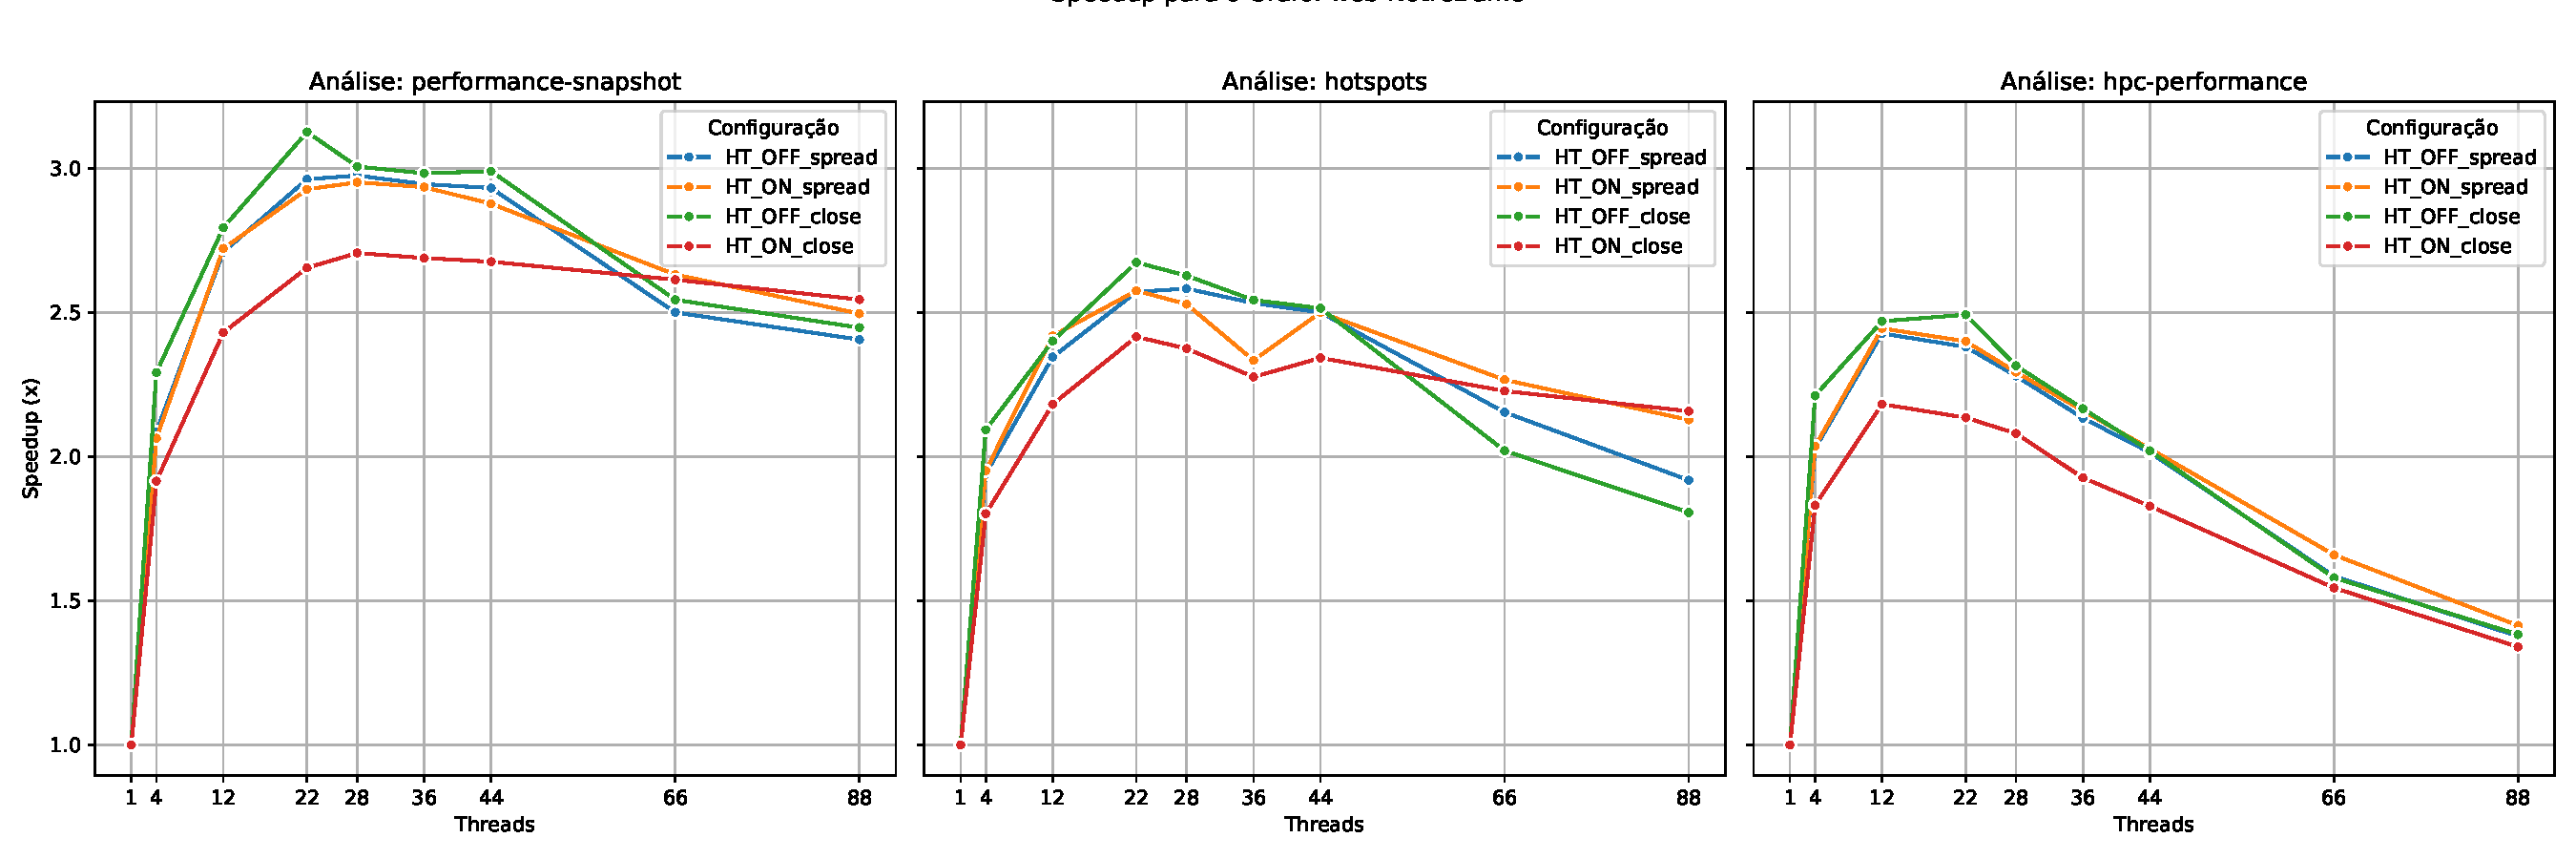
\includegraphics[width=0.95\paperwidth]{graficos/speedup_web-NotreDame.pdf}
        }        
    \end{figure}
    \centering
    A HT\_OFF\_close se saiu muito bem com poucas threads, obtendo o maior speedup.
\end{frame}

\begin{frame}
    \frametitle{Speedup - Stanford}

    \begin{figure}
        \centering
        \makebox[\textwidth][c]{%

            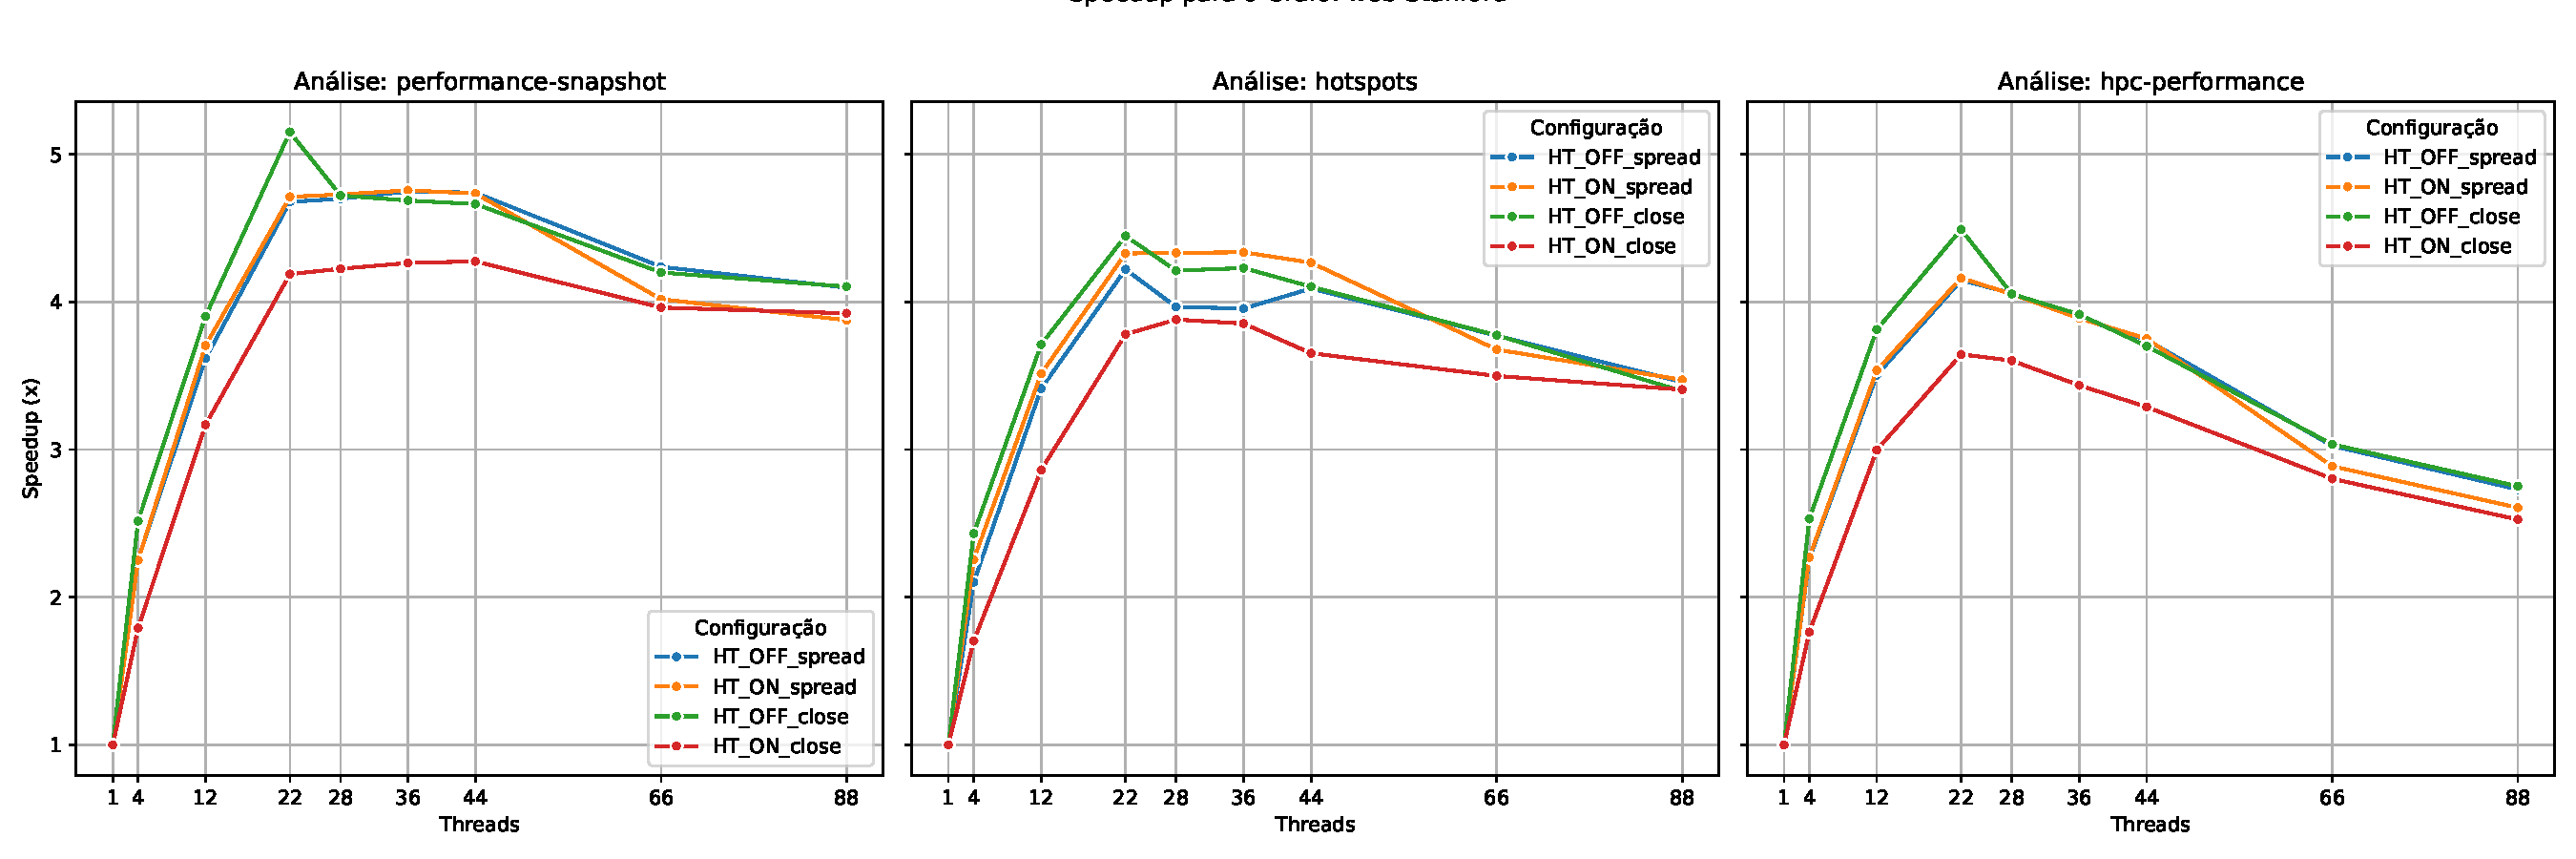
\includegraphics[width=0.95\paperwidth]{graficos/speedup_web-Stanford.pdf}
        }        
    \end{figure}
    \centering
    Novamente, a HT\_OFF\_close obteve o melhor speedup com poucas threads.
\end{frame}

\begin{frame}[fragile]
    \frametitle{Melhores Configurações de Speedup (Parte 1)}
    
    % Usando o ambiente 'center' para garantir a centralização
    \begin{center}
    \scriptsize 
    \setlength{\tabcolsep}{4pt} 
    
    \begin{tabular}{@{}llrccr@{}}
        \toprule
        \textbf{Grafo} & \textbf{Análise} & \textbf{Threads} & \textbf{HT} & \textbf{Bind} & \textbf{Speedup} \\
        \midrule
        \multirow{3}{*}{com-Friendster} & hotspots & 22 & True & close & 5.71 \\
         & hpc & 28 & True & close & 6.08 \\
         & snapshot & 22 & True & close & 5.68 \\
        \midrule
        \multirow{3}{*}{com-LiveJournal} & hotspots & 36 & True & spread & 2.55 \\
         & hpc & 12 & True & spread & 2.38 \\
         & snapshot & 44 & False & spread & 3.11 \\
        \midrule
        \multirow{3}{*}{com-Orkut} & hotspots & 88 & True & close & 2.56 \\
         & hpc & 36 & True & close & 2.35 \\
         & snapshot & 88 & True & close & 2.70 \\
        \midrule
        \multirow{3}{*}{web-BerkStan} & hotspots & 36 & False & close & 3.90 \\
         & hpc & 36 & True & spread & 3.72 \\
         & snapshot & 36 & False & spread & 4.19 \\
        \bottomrule
    \end{tabular}
    \end{center} 
\end{frame}

\begin{frame}[fragile]
    \frametitle{Melhores Configurações de Speedup (Parte 2)}
    
    % Usando o ambiente 'center' para garantir a centralização
    \begin{center}
    \scriptsize 
    \setlength{\tabcolsep}{4pt} 
    
    \begin{tabular}{@{}llrccr@{}}
        \toprule
        \textbf{Grafo} & \textbf{Análise} & \textbf{Threads} & \textbf{HT} & \textbf{Bind} & \textbf{Speedup} \\
        \midrule
        \multirow{3}{*}{web-Google} & hotspots & 66 & True & close & 6.39 \\
         & hpc & 22 & False & close & 5.89 \\
         & snapshot & 66 & True & close & 6.93 \\
        \midrule
        \multirow{3}{*}{web-NotreDame} & hotspots & 22 & False & close & 2.67 \\
         & hpc & 22 & False & close & 2.49 \\
         & snapshot & 22 & False & close & 3.13 \\
        \midrule
        \multirow{3}{*}{web-Stanford} & hotspots & 22 & False & close & 4.45 \\
         & hpc & 22 & False & close & 4.49 \\
         & snapshot & 22 & False & close & 5.15 \\
        \bottomrule
    \end{tabular}
    \end{center} 
\end{frame}

\begin{frame}
    \frametitle{Explicação dos Gráficos de Eficiência Paralela}
        Agora, mostraremos os gráficos de eficiência paralela.
        A eficiência paralela é uma maneira de quantificar o quão bem foram utilizados os recursos de \textit{hardware} no paralelismo.

        Ela pode ser calculada pela seguinte fórmula:
        
        $$ E_p = \frac{T_s}{(N \times T_p)} $$
    
        Onde:
        \begin{itemize}
            \item[$E_p$] é a eficiência paralela.
            \item[$T_s$] é o tempo de execução sequencial (com 1 thread).
            \item[$N$] é o número de threads utilizados.
            \item[$T_p$] é o tempo de execução paralelo com N threads.
        \end{itemize}
        
        \vspace{\fill} % Empurra o texto seguinte para o final do slide
        
        Os gráficos a seguir estão organizados similarmente aos últimos.
\end{frame}

\begin{frame}
    \frametitle{Eficiência Paralela - Friendster}

    \begin{figure}
        \centering
        \makebox[\textwidth][c]{%

            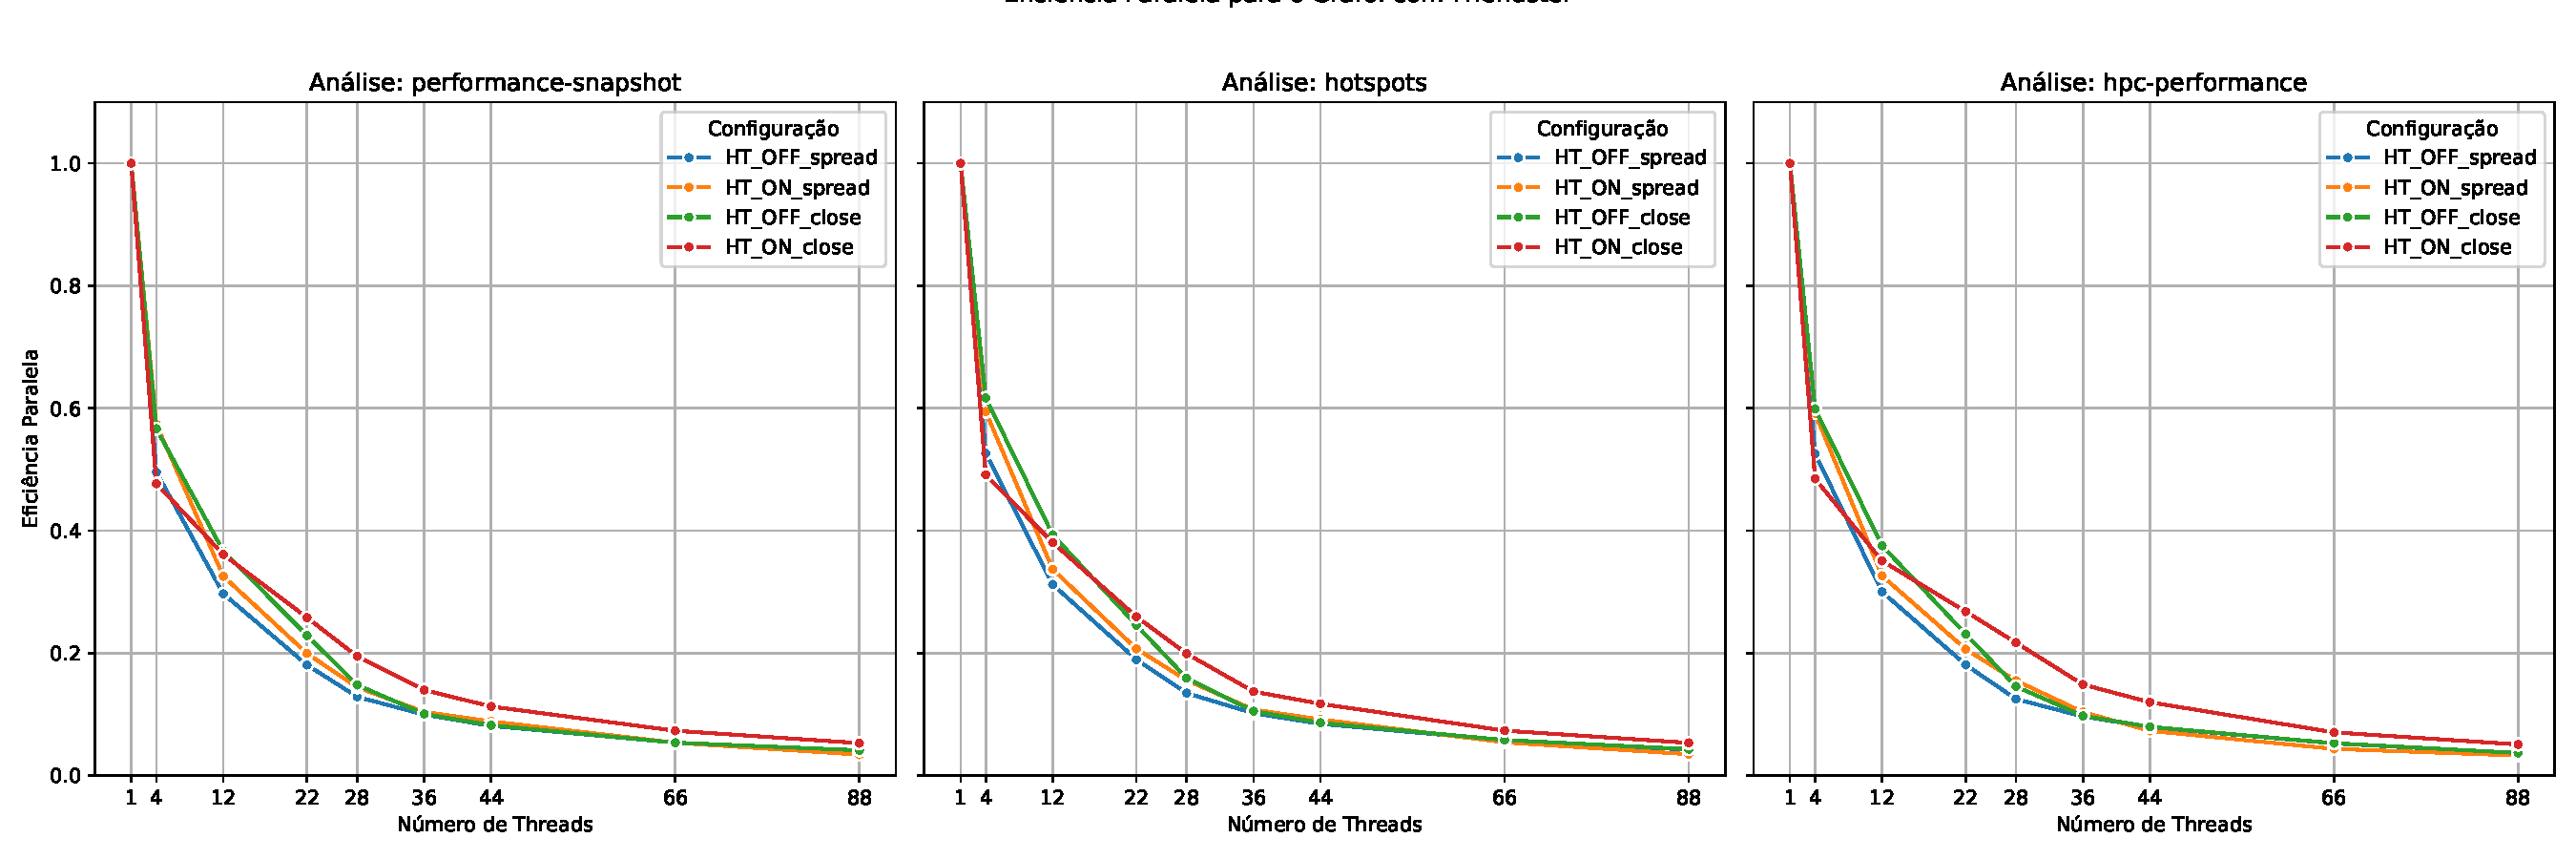
\includegraphics[width=0.95\paperwidth]{graficos/parallel_efficiency_com-Friendster.pdf}
        }        
    \end{figure}
\end{frame}

\begin{frame}
    \frametitle{Eficiência Paralela - LiveJournal}

    \begin{figure}
        \centering
        \makebox[\textwidth][c]{%
            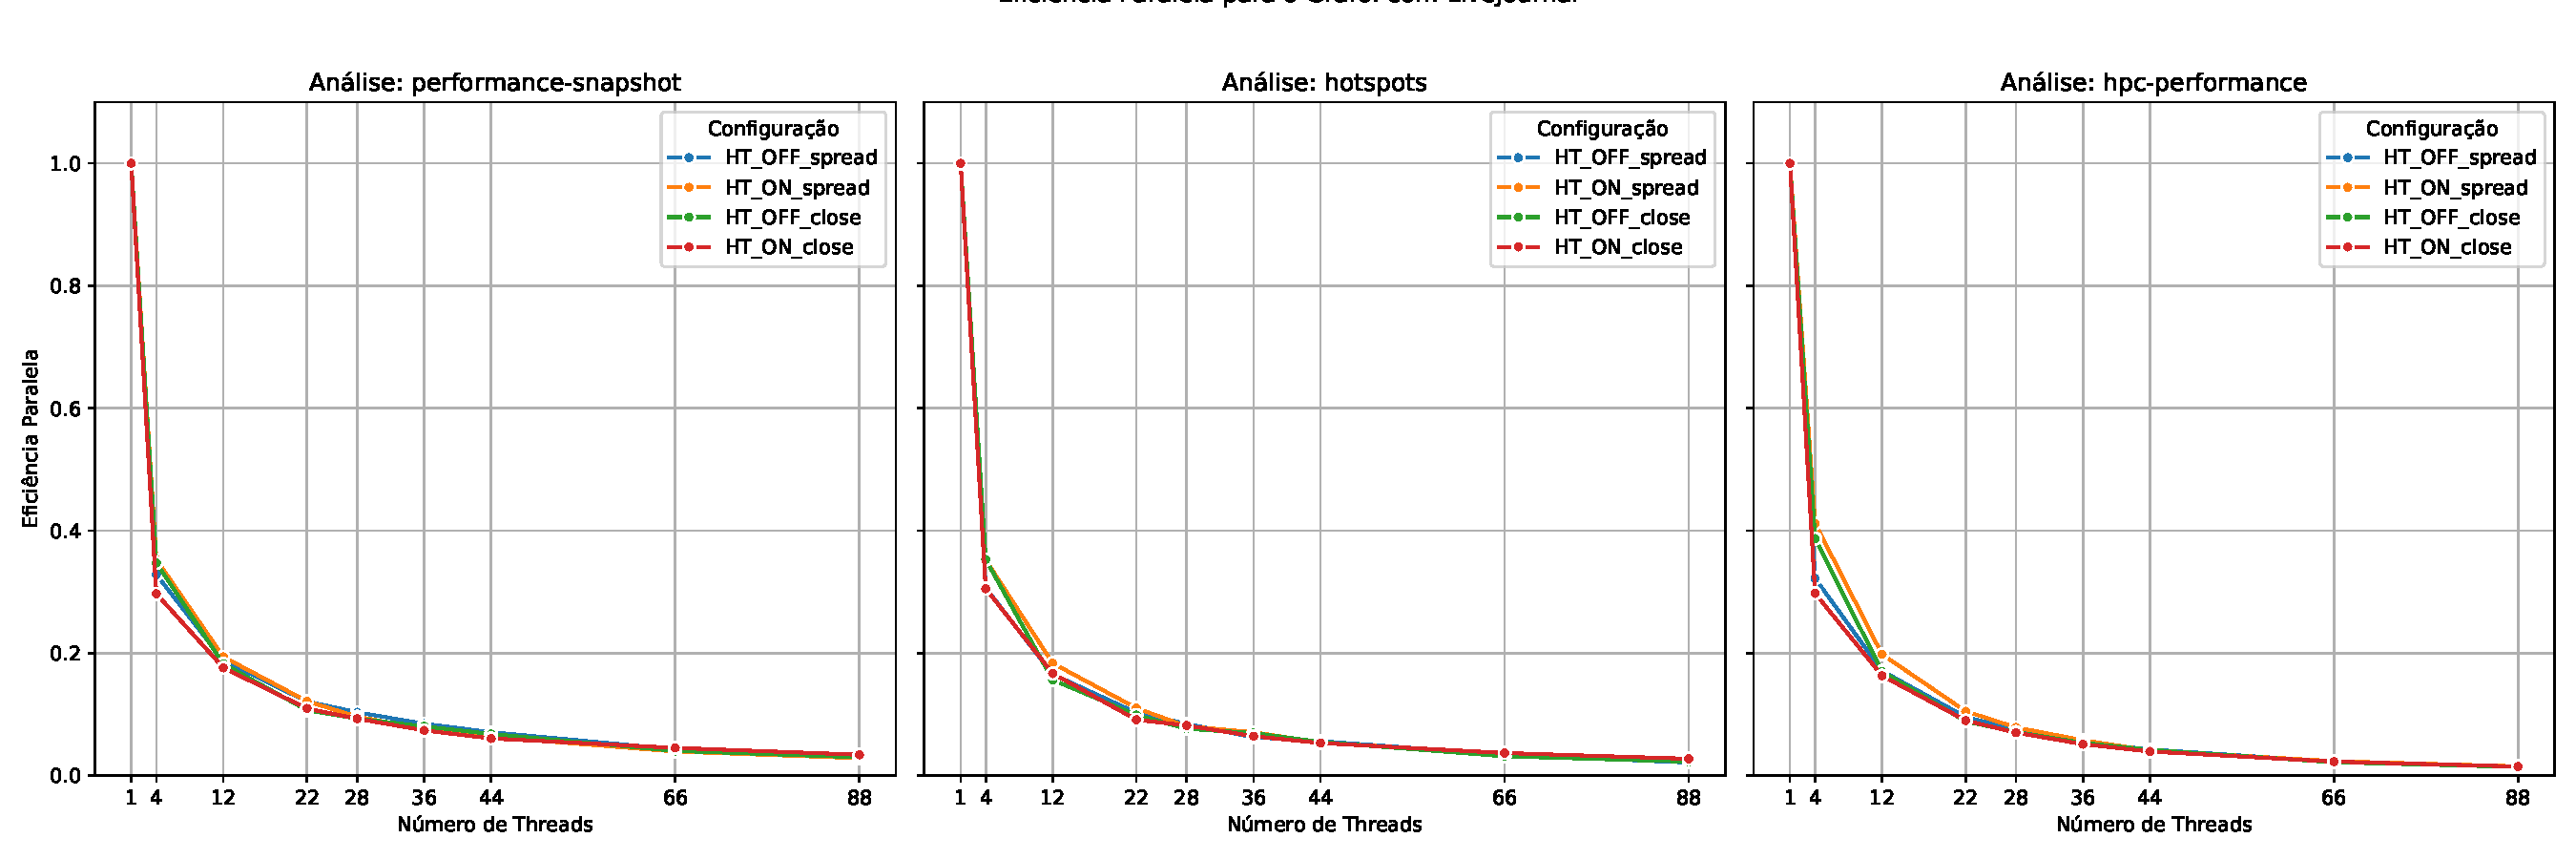
\includegraphics[width=0.95\paperwidth]{graficos/parallel_efficiency_com-LiveJournal.pdf}
        }        
    \end{figure}
\end{frame}

\begin{frame}
    \frametitle{Eficiência Paralela - Orkut}

    \begin{figure}
        \centering
        \makebox[\textwidth][c]{%

            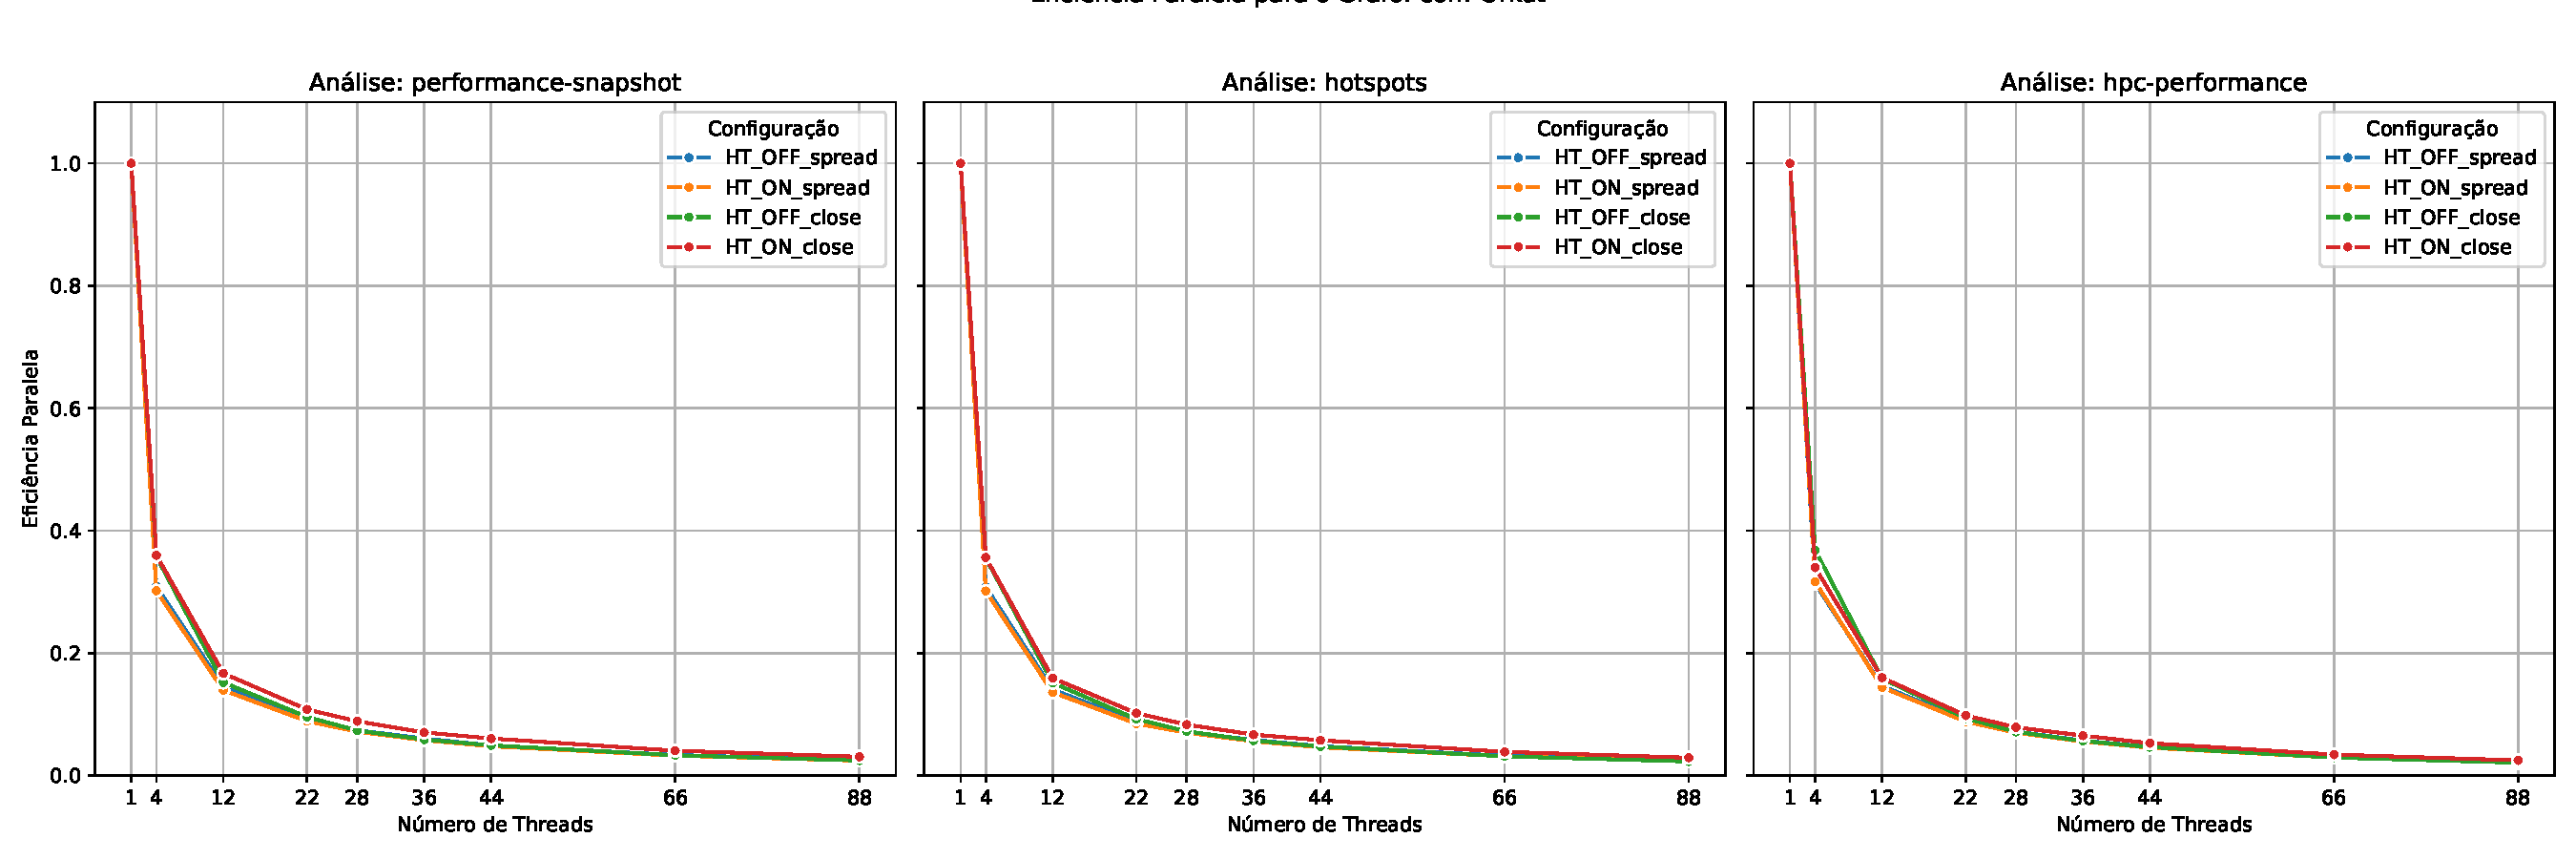
\includegraphics[width=0.95\paperwidth]{graficos/parallel_efficiency_com-Orkut.pdf}
        }        
    \end{figure}
\end{frame}

\begin{frame}
    \frametitle{Eficiência Paralela - BerkStan}

    \begin{figure}
        \centering
        \makebox[\textwidth][c]{%

            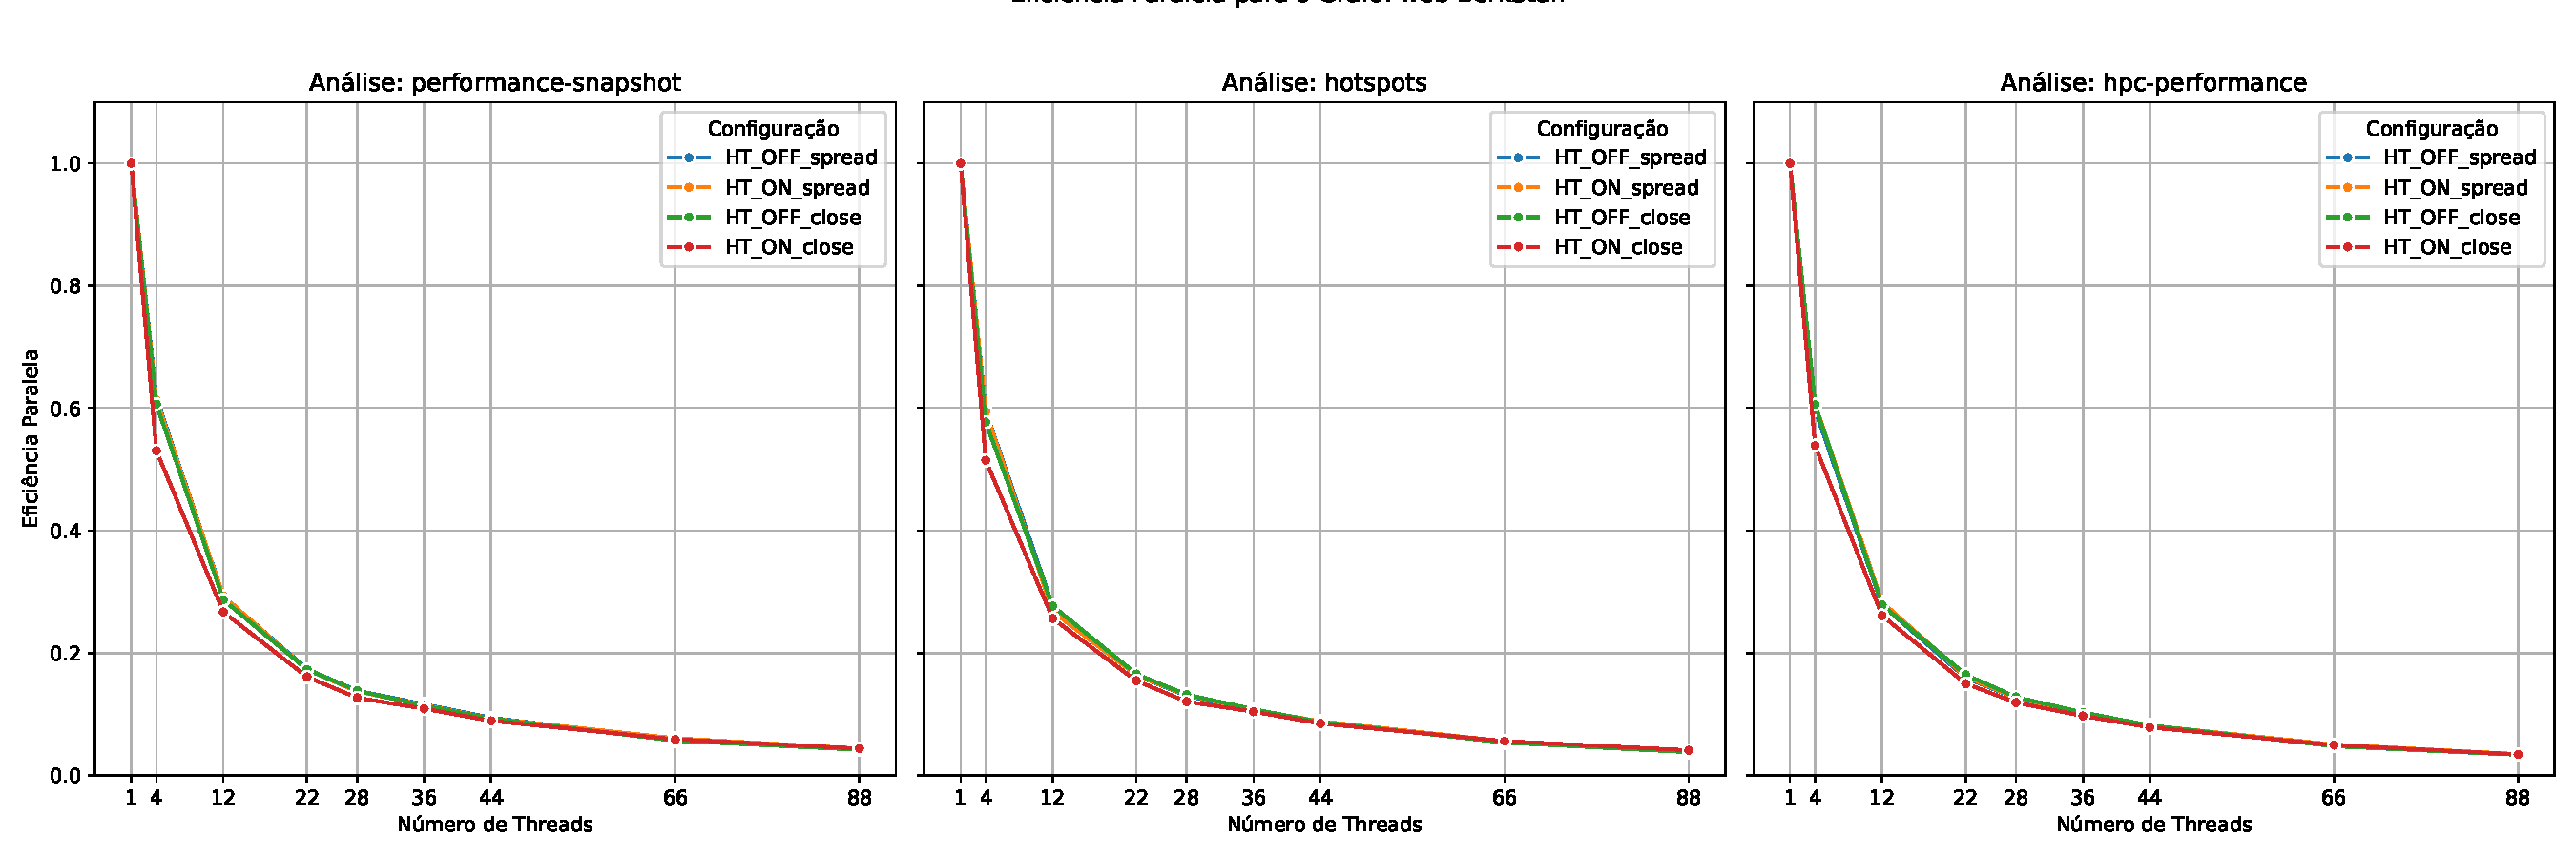
\includegraphics[width=0.95\paperwidth]{graficos/parallel_efficiency_web-BerkStan.pdf}
        }        
    \end{figure}
\end{frame}

\begin{frame}
    \frametitle{Eficiência Paralela - Google}

    \begin{figure}
        \centering
        \makebox[\textwidth][c]{%

            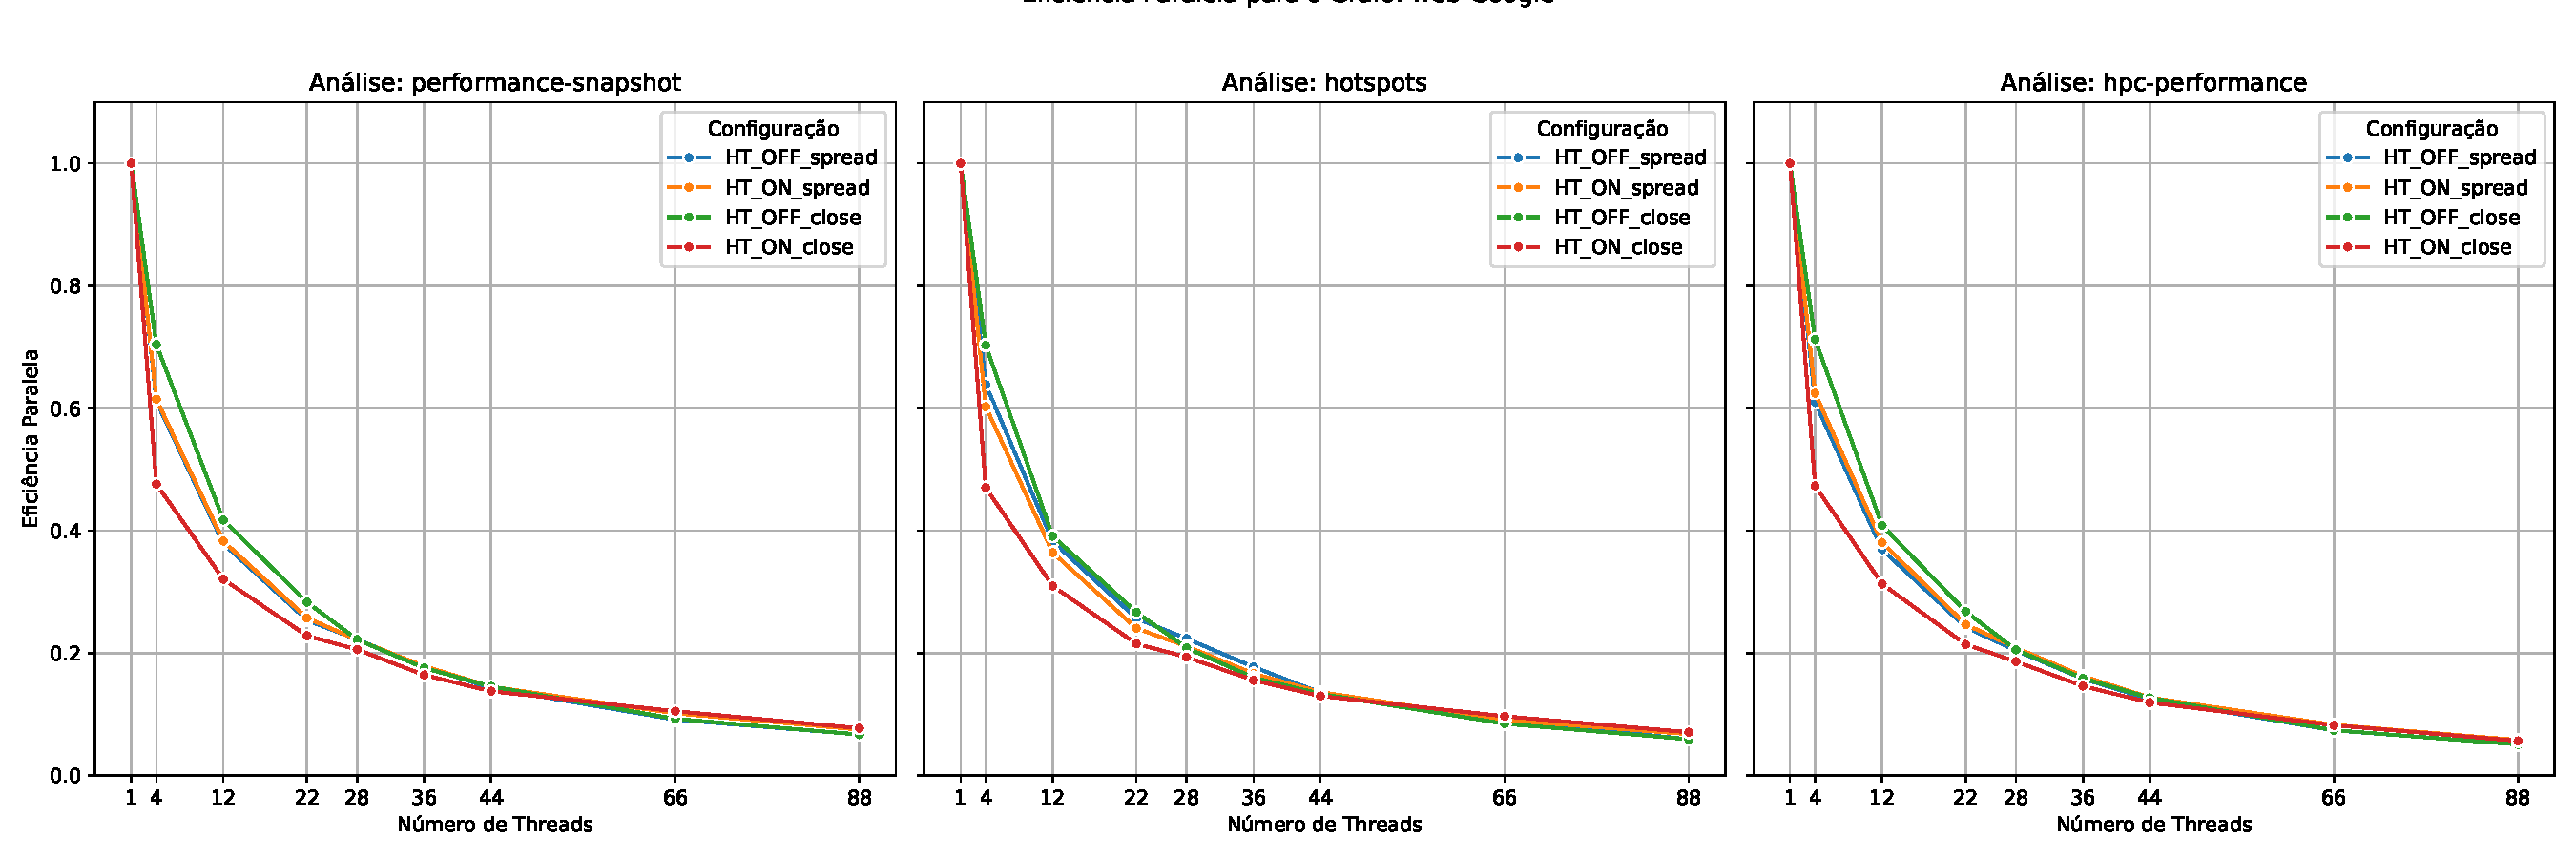
\includegraphics[width=0.95\paperwidth]{graficos/parallel_efficiency_web-Google.pdf}
        }        
    \end{figure}
\end{frame}

\begin{frame}
    \frametitle{Eficiência Paralela - NotreDame}

    \begin{figure}
        \centering
        \makebox[\textwidth][c]{%

            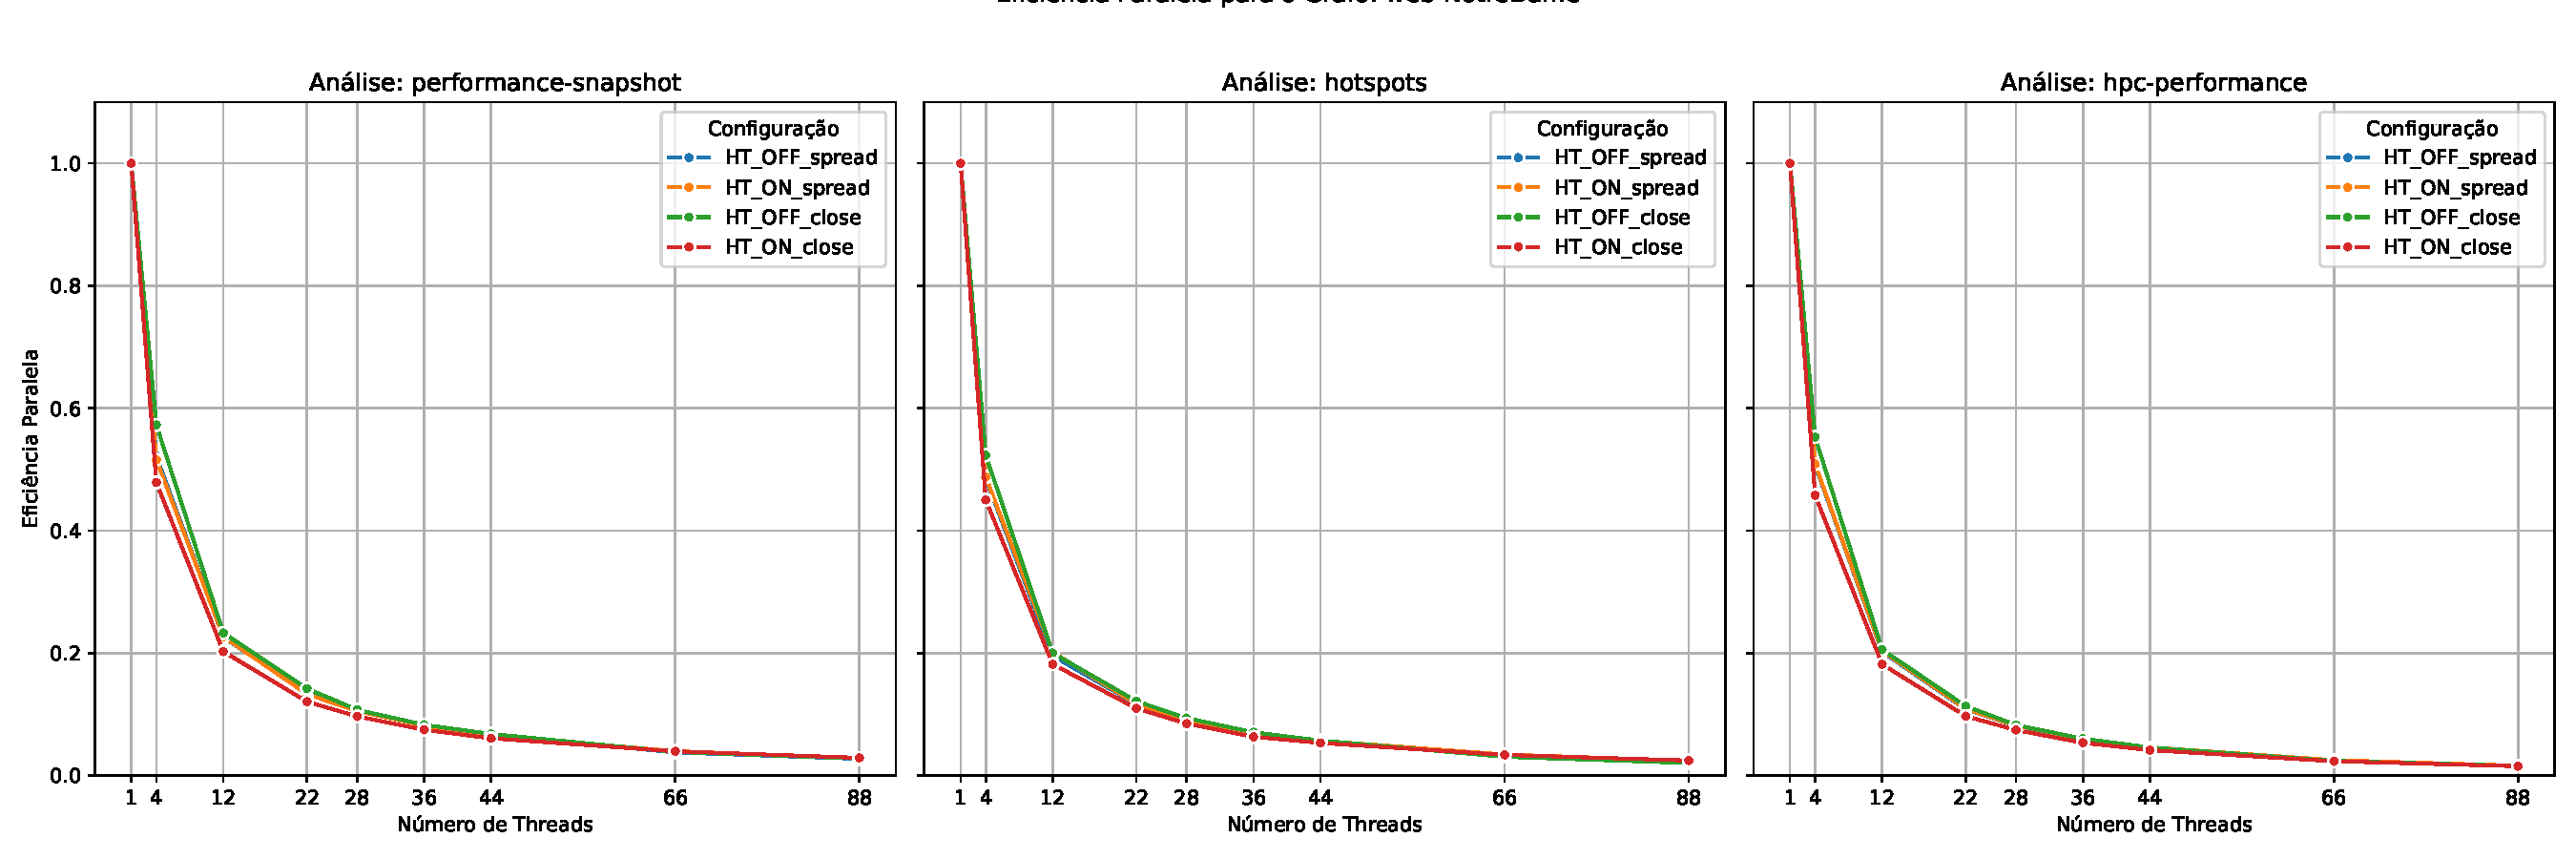
\includegraphics[width=0.95\paperwidth]{graficos/parallel_efficiency_web-NotreDame.pdf}
        }        
    \end{figure}
\end{frame}

\begin{frame}
    \frametitle{Eficiência Paralela - Stanford}

    \begin{figure}
        \centering
        \makebox[\textwidth][c]{%

            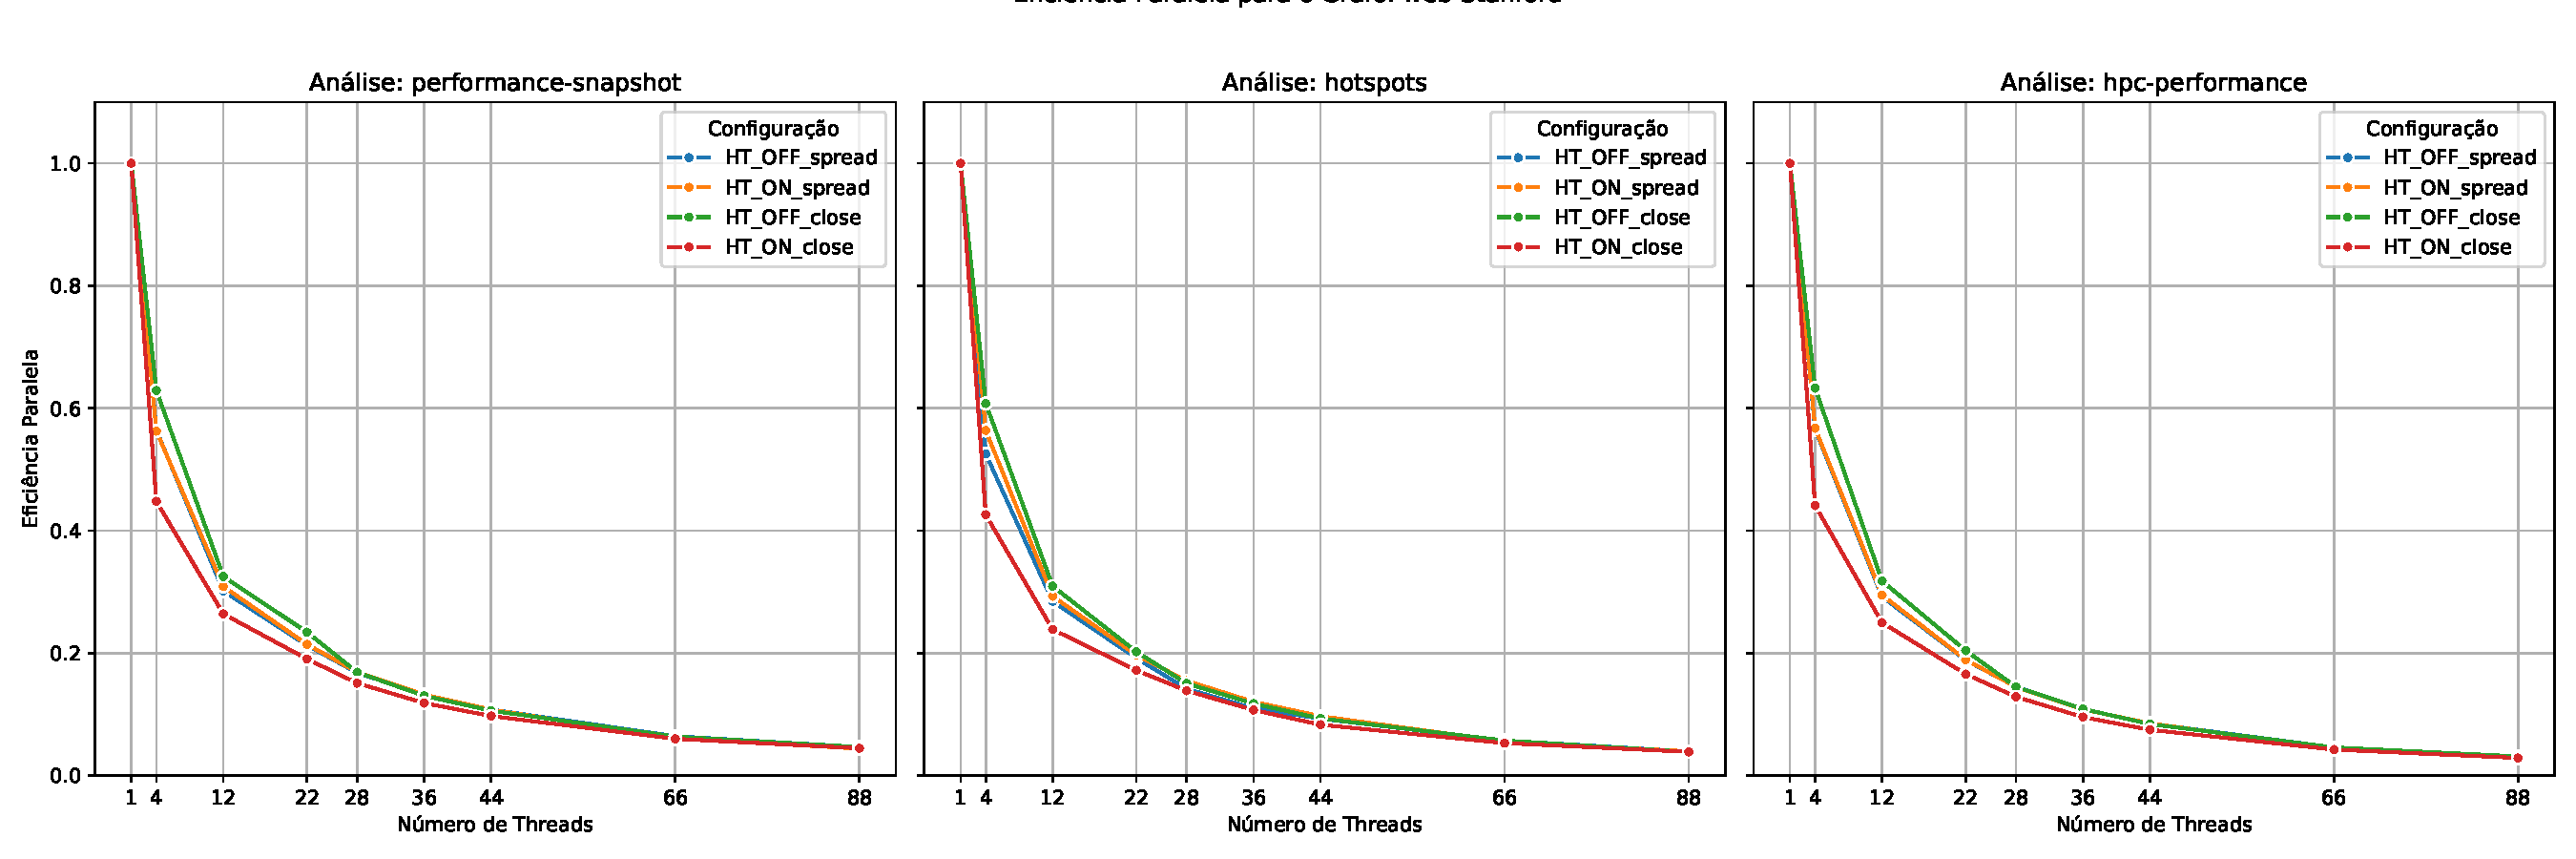
\includegraphics[width=0.95\paperwidth]{graficos/parallel_efficiency_web-Stanford.pdf}
        }        
    \end{figure}
\end{frame}

\section{Dificuldades}
\begin{frame}{Dificuldades enfrentadas}
 \begin{itemize}
     \item Vtune gerando muitos dados, a grande maioria não eram de interesse do grupo.
     \item Falta de disponibilidade da máquina. \\ ( Obrigado bmmoreira! )
     \item Conseguir deixar executando sem o Hyperthreading.
     \item Vtune gerando arquivos de saída mal formatados e grandes.
     
 \end{itemize}    
\end{frame}

\section{Conclusão}
\begin{frame}{Conclusão do Projeto}
Mesmo com essa análise superficial, já conseguimos chegar a algumas conclusões:
 \begin{itemize}
     \item A política de binding de threads "close" consegue aproveitar muito bem a localidade de dados com muitas threads, mas com poucas threads essa eficiência não se reproduz.
     \item A presença de Hyperthreading produz diferenças significativas no speedup das aplicações, mas também houve casos onde estar com ele desligado tornava o código mais rápido.
     \item E o mais importante: \textbf{Não há configuração global pra nenhuma das entradas que cause o maior speedup!}
     
 \end{itemize}    
\end{frame}

\section{Próximos passos}
\begin{frame}{Perspectiva do projeto}
 \begin{enumerate}
     \item Começar a trabalhar no documento final de entrega do projeto (com o \textit{template} em \LaTeX providenciado pelo professor).
     \item Começar a analisar o resto dos dados providenciados pelo Intel VTune, como uso dos núcleos físicos e lógicos, frequência média do processador, se é a memória que limita o desempenho, etc.
     \item Finalmente, completar nosso \textit{Notebook} utilizado com novos gráficos e novas análises.
 \end{enumerate}
 \tiny % Deixa a fonte bem pequena
    Todos dados disponíveis no repositório: \url{https://github.com/thgdsg/perf-analysis}
\end{frame}

\section*{}
\begin{frame}
    \frametitle{Obrigado!}
    \InfContacts
\end{frame}

\end{document}